\chapter{Umsetzung}

Im folgenden Kapitel wir die Umsetzung der Ziele aus dem vorigen Kapitel behandelt. Zuerst wird die Elektronik behandelt, danach das Gassystem und abschließend das Wirbelbett und die Testergebnisse.


\section{AP 1 - Analyse}

\paragraph{Elektronik}
\hfill \\
Der Hautschwachpunkt der Elektronik ist die Verkabelung, da man es bei dem Setup mit mehreren Teilen zu tun hat, die teils verlötet, teils gesteckt werden. Das führt zu einem insgesamt sensiblen Aufbau. Ziel muss es also sein, so viele Kabel wie möglich geeignet zu verpacken, sodass sie möglichst wenig äußeren Einflüssen ausgesetzt sind. 


\paragraph{Gassystem}
\hfill \\
Eine Herstellerauswahl hat hier nicht stattgefunden, da bereits vorhandene Verrohrung der Firma Swagelok weitergenutzt werden sollte. Dies hatte auch den Vorteil, das ein Berater aus dem nahegelegenen Standort Düsseldorf bei der Auslegung und Wahl der Komponenten beraten konnte. \\
Insgesamt wir der Aufbau des Gassystems und Luftbefeuchters knapp \SI{1600}{\euro} kosten, wenn man dabei nur die zusätzlich bestellten Materialien einbezieht und nicht die ohnehin vorhandenen. Der größte Teil der Kosten fällt dabei auf den Flowcontroller zurück. Eine genaue Aufstellung ist im folgenden zu sehen:

\begin{center}
	\begin{tabular}{|l|S|S|S|}
		{Teil}  & {Anzahl} & {Kosten/Stück} & {Kosten} \\
		\hline
		&       &       &  \\
		{Flowcontroller} & 1     & 1186,00  & 1186,00 \\
		{Mutter mit Ferrul} & 10    & 4,80   & 48,00 \\
		{Kükenhahn} & 3     & 69,25 & 207,75 \\
		{T-Stück} & 2     & 26,11 & 52,22 \\
		{Verbinungsstück} & 1     & 12,87 & 12,87 \\
		{Endanschluss} & 4     & 12,87 & 51,48 \\
		{Buna N Schlauch} & 9     & 2,67  & 24,03 \\
		{Einschraubverbindung M12x1} & 3     & 16,67 & 50,01 \\
		{Teichnetz} & 1     & 8,45  & 8,45 \\
		{Küchenschwämme} & 3     & 2,99  & 8,97 \\
		\hline 
		&       &       &  \\
		{Summe} &       &       & 1632,36 \\
	\end{tabular}
\end{center}


\paragraph{Wirbelbett}
\hfill \\
Bei der Analyse des bisherigen Wirbelbettes wurde klar, das die Bauhöhe, neben der Dichtheit, ein entscheidendes Kriterium ist. Die Bauhöhe ist durch den Lichtstreuaufbau nach begrenzt und enthält eine Mindesthöhe über dem Rotationsarm und eine Maximalhöhe, da der Aufbau sonst gegen Stahlträger stößt. Daraus folgte unmittelbar, das die Anschlüsse für Luft und Ionisator beide seitlich, also in der horizontalen Ebene erfolgen müssen. \\
Weiterhin wurde beschlossen den Justiermechanismus des alten Aufbaus weiterzuverwenden, da dieser bereits funktioniert und leicht in den neuen Aufbau integriert werden kann. 


\newpage

\section{AP 2 - Elektronik}

\paragraph{Anforderungen}
\hfill \\
Bei der Elektronik gab es zwei verschiedene Bereiche: \\
In einem ersten Schritt sollte ein A-D\footnote{Analog-Digital} Wandler gefunden werden, mit dem der Drucksensor mit \SI{0,1}{mbar} Genauigkeit ausgelesen werden kann. Zum Start es Projekts wurde der Drucksensor über das $\SI{10}{bit}$ breite analoge Interface des Arduino ausgelesen. Das ist für eine genaue Auswertung der Experimente zu wenig. Der A-D Wandler soll zwischen den Drucksensor und den Arduino geschaltet werden, damit die Auslesegenauigkeit von \SI{0,1}{mbar} erreicht werden kann. Der Drucksensor hat einen Messbereich von \SIrange{0}{2}{\bar} absolut und gibt diesen auf \SIrange{0}{10}{\volt} aus. Da der Arduino maximal $\SI{5}{V}$ als Eingangsspannung verarbeiten kann, wird die Spannung über einen Spannungsteiler auf \SIrange{0}{5}{\volt} reduziert und dann eingelesen. 
Als Resultat soll die gesamte Elektronik als \glqq Blackbox\grqq \ vorliegen, sodass man nach außen hin nur noch Anschlüsse hat, die klar gekennzeichnet sind. Dies soll in Form eines Gehäuses erledigt werden, das zudem auch noch rudimentären Schutz gegen Schmutz bietet.


\subsection{Umsetzung}


\paragraph{Elektronik}
\hfill \\
Der Arduino bietet einen SPI\footnote{\url{http://www.mct.de/faq/spi.html}} Bus zum Anschluss von externen Modulen an. Darüber können die digitalen Outputdaten der angesteckten Module ausgelesen werden, unabhängig davon wie hoch die Auflösung der Module ist. Auf Grund dessen wurde entschieden ein Modul für diesen Bus zu verwenden und aus Gründen der Genauigkeit wurde sich für ein \SI{16}{bit} Modul entschieden. \\
Damit kann man mit einer Genauigkeit von $\frac{\SI{5}{V}}{\SI{65536}{bit}} = \SI{0,00008}{V/bit}$ die Ausgangsspannung des Drucksensors auslesen. Das bedeutet auch eine Auslesegenauigkeit von $\frac{\SI{1250}{mbar}}{\SI{65536}{bit}} = \SI{0,02}{mbar/bit}$. \\
Zur Auswahl standen zwei verschiedene A-D Wandler:

\begin{center}
\begin{tabular}{l|c|c}
	& TM7705 Dual 16-bit ADC & AD420 \\ 
	\hline Preis [\euro]	& 15  & 7 \\ 
	\hline Auflösung [bit]	& 16  & 16 \\ 
	\hline Power supply [Volt]	& 1,3/3/5  & 12-32 \\ 
	\hline Lieferzeit [Wochen]	& 3  & 3 \\ 
	\hline Montage 	& auf Platine  & nur Chip \\ 
\end{tabular} 	
\end{center}


Es wurde sich für den TM7705 Dual 16-bit ADC entschieden, da dieser bereits auf eine Platine aufgelötet ist und somit ohne zusätzliche Arbeiten verwendet werden kann und zudem auch direkt vom Arduino mit Spannung versorgt werden kann. Der AD420 hätte ein zusätzliches Netzteil gebraucht, was wiederum mehr Platz in Anspruch genommen hätte. Schematisch ist die Schaltung mit dem A-D Wandler die unten stehende:


\begin{figure}[h]
	\begin{center}
		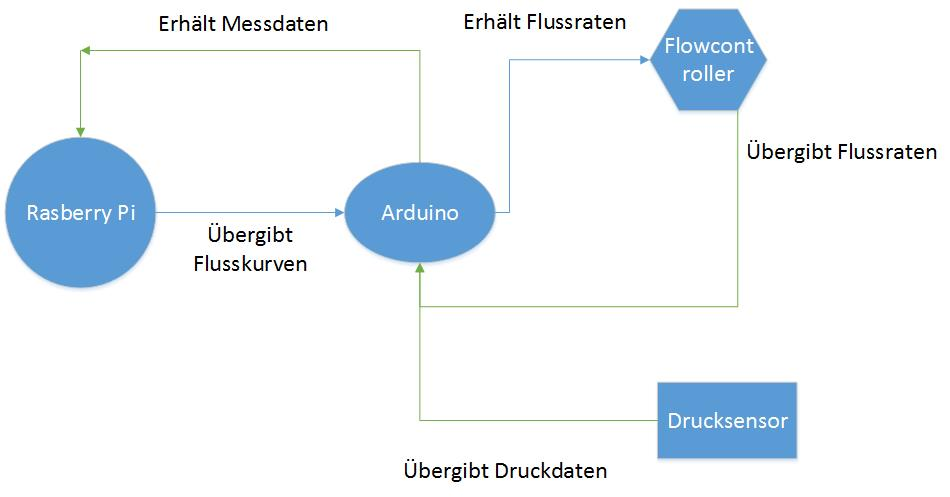
\includegraphics[scale=0.6]{Schema_Elektronik.jpg}
		\caption{Schema Elektronik}
	\end{center}
\end{figure}


\paragraph{Gehäuse (still in progress)} 
\hfill \\
Da es insbesondere im Lichtstreuaufbau nur sehr begrenzten Stauraum gibt und sämtliche Bauteile, das Wirbelbett selbst ausgenommen, auf einer Platte verbaut werden sollen, wurde gegen ein kommerziell erhältliches Gehäuse entschieden. \\ 
Stattdessen wurde ein Gehäuse entworfen, in dem sowohl der Arduino als auch das Board mit dem Spannungsteiler passgenau Platz finden. Dabei wurde darauf geachtet, dass die Kontakte unterhalb des Arduinos und des Boards genug Platz haben, sodass es keinerlei unbeabsichtigte Reibung der Komponenten am Gehäuse gibt. \\
Für die Anschlüsse wurden möglichst kleine Löcher im Gehäuse gelassen, sodass ein größtmöglicher Schutz gegen Schmutz bei größtmöglichem Komfort gewährleistet wird. \\
Beim Deckel wurde sich für eine Presspassung entschieden, zudem dient der Deckel gleichzeitig dazu die Komponenten innerhalb des Gehäuses an Ort und Stelle zu halten. Dies wurde über Streben, die vom Deckel nach unten bis auf die jeweilige Komponente geht realisiert.

Hier Bilder einfügen!!

\newpage

\section{AP3 - Gassystem}

\subsection{Anforderungen}

Beim Gassystem soll neben der Luftdichtheit auch eine mechanische Stabilität erreicht werden, damit es einfach von zwischen Normalem und Lichtstreubaufbau transportiert werden kann. Außerdem soll der Gasstrom von \SIrange{0}{120}{l/h} auf \SIrange{0}{3000}{l/h} erhöht werden. Zudem sollen die Werte, die der Drucksensor vor und hinter dem Wirbelbett misst um weniger als \SI{1}{\%} differieren. Weiterhin muss das gesamte Gassystem mit Luftbefeuchter in den Lichtstreuaufbau passen. \\
Der Luftbefeuchter selbst soll im Betrieb eine Luftfeuchtigkeit von \SI{75}{\%} erreichen und den gesamten Regelbereich des Flowcontrollers abdecken.



\subsection{Umsetzung}

\subsubsection{Flowcontroller}

Aus den Tabellen im Abschnitt \glqq Ziele der Arbeit\grqq \ folgt, das ein Gasfluss von \SIrange{0}{3000}{l/h} alle Anforderungen erfüllt. \\
Es gab mehrere Lösungsarten diese Anforderung zu erfüllen. Eine Lösung bestand darin, den Luftstrom über mehrere Gasdurchflussbegrenzer und Ventile auf definierte Werte voreinzustellen und mit dem vorhandenen Flowcontroller von da ab zu regeln. Zudem kann man einen Massenstromregler kaufen, der komplett digital zu regeln ist. \\
Die erste Lösungsart wurde verworfen, weil es sich als zu ungenau und nicht deutlich billiger in Aufwand und Kosten darstellte. Zudem wäre der Aufbau deutlich größer gewesen. Die Lösung bestand somit darin einen neuen Flowcontroller anzuschaffen, der den gesamten Regelbereich mit einer hinreichenden Genauigkeit abdeckt und gleichzeitig gut in das Gassystem integriert werden kann. Dazu wurden zwei Angebote eingeholt, die im folgenden dargelegt sind:


\begin{tabular}{l|c|c}
	 & Brooks & Bronkhorst \\ 
	\hline Regelbereich & \SIrange{0}{3000}{l/h} & \SIrange{0}{3000}{l/h} \\ 
	\hline Genauigkeit $20 - \SI{100}{\%}$ & $\pm \SI{0,9}{\%}$ Istwert & $\pm \SI{0,5}{\%}$ Istwert $+ \pm \SI{0,1}{\%}$ Endwert\\ 
	\hline Genauigkeit $0 - \SI{20}{\%}$ & $\pm \SI{0,18}{\%}$ Istwert & $\pm \SI{0,5}{\%}$ Istwert $+ \pm \SI{0,1}{\%}$ Endwert \\ 
	\hline Preis in \euro & 1187,33 & 1382,66 \\ 
\end{tabular} 

\vspace{0,5cm}

Es wurde sich für den Flowcontroller der Firma Brooks entschieden. Das geschah aus mehreren Gründen: \\
Im ursprünglichen Aufbau war auch ein Flowcontroler von Brooks verbaut, daher war bekannt wie dieser angesteuert wird und hatten bereits den benötigten Stecker. Weiterhin ist die Genauigkeit des Brookscontrollers im niedriegen Regelbereich besser als die des Bronkhorstcontrollers. Dies ist grade bei quantitativen Messungen mit kleinen Rohrdurchmessern und sehr feinen granularen Medien essentiell. \\
Zudem waren die Anschaffungskosten für den Brookscontroller um ca $\SI{200}{Euro}$ niedriger. Außerdem hatte die Gruppe bei einem anderen Controller von Bronkhorst einige Probleme mit der Zuverlässigkeit gehabt, während der Brooks Controller keine aufwies.


\subsubsection{Verrohrung}

Um die geforderte Stabilität und Reproduzierbarkeit zu gewährleisten, wurde entschieden das gesamte Gassystem aus Stahlrohren (\textcolor{blue}{blau}) zu bauen. Das bietet, neben der besseren Luftdichtigkeit, auch einen höheren Schutz gegenüber äußeren Umwelteinflüssen wie ätzenden Flüssigkeiten oder herunterfallenden Gegenständen.
Auf der Skizze in Abbildung xy kann man das gebaute System sehen:
\hfill \\

\begin{figure}[h]
	\begin{center}
		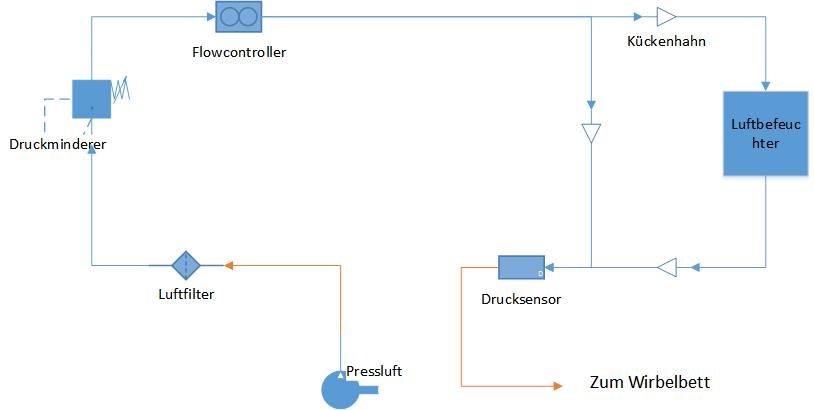
\includegraphics[scale=0.6]{Aufbau_Gassystem.jpg}
		\caption{Schema Gassystem}
	\end{center}
\end{figure}


Um dem Aufbau die nötige Flexibilität zu geben, die beim Umbau zwischen den beiden Versuchsständen nötig ist, wurde das Wirbelbett mit einem Bunaschlauch (\textcolor{orange}{orange}) an das Gassystem angeschlossen. Der Bunaschlauch gewährleistet neben der nötigen Flexibiltät auch eine deutlich verminderte Knickgefahr, da der Schlauch aus dickem Gummi mit zusätzlicher Verstärkung aus Rayongewebe besteht.
Um Problemen mit dem Flowcontroller zu begegnen, wird das Gassystem über eine Druckluftflasche mit einstellbarem Ausgangsdruck gespeist. Sämtliche Rohrleitungen ab dem Luftfilter bis zum Übergang zum Wirbelbett sind aus Edelstahl. \\
Die Ventile, T-Stücke und Verbindungsstücke sind auch aus Edelstahl, da Messing zwar billiger wäre, allerdings auch weicher, was zu Verformungen und höherem Verschleiß führen kann. Zur weiteren Erhöhung der Stabilität und Reproduzierbarkeit wurde das System zudem auf einer Holzplatte befestigt. \\
Abschließend kann gesagt werden, das durch die Wahl der Verrohrung ein luftdichtes Gassystem erreicht wurde. Außerdem ist der Aufbau mit $\SI{0,41}{m} \cdot \SI{0,33}{m}$ passend für den Lichtstreuaufbau.


\subsubsection{Luftbefeuchter}

Um die Anforderungen für den Luftbefeuchter zu erfüllen, wurden drei mögliche Lösungen geprüft, dabei waren die Größe und die Kosten der Lösung das Hauptaugenmerk. \\
Von Swagelok gibt es eine Lösung ähnlich dem jetzigen Drucksensor. Über ein spezielles Rohrverbindungsstück kann ein Metallzylinder angeschlossen werden, der senkrecht auf dem Rohr nach oben steht. Dieser wird mit Wasser gefüllt, das von unten mit Luft durchströmt wird und die anschließend oben abgenommen und Richtung Wirbelbett fließt. \\
In einer anderen Arbeit \cite{Fallturmexperiment} wurde die Luftbefeuchtung realisiert, indem man Luft direkt an einer  Wasseroberfläche vorbeiströmen ließ und die Luft durch Diffusion Wasser aufnahm. \\
Eine alternative Methode besteht darin einen eigenen Luftbefeuchter zu bauen, mit gleicher Funktion wie die Lösung von Swagelok. 


\paragraph{Auswahl}

\hfill \\

Es wurde sich für die Lösung Eigenbau entschieden, da die anderen Methoden Mängel aufweisen. Die Lösung von Swagelok ist zum einen sehr teuer, zudem würde bei abgeschaltetem Gasfluss Wasser in das System fließen. \\
Die Methode des Vorbeiströmens wurde verworfen, weil eine zu große Strömfläche gebraucht wurde. Anhand der Formeln aus der Arbeit von Herrn Schmitz, erhielt man eine Fläche von $\SI{50}{cm} \cdot \SI{50}{cm}$. Einen Aufbau dieser Größe kann man nicht im Lichtstreuaufbau unterbringen.

\paragraph{Umsetzung}

\hfill \\

Damit der Befeuchter in den Lichtstreuaufbau passt, wurde zu Anfang ein Behältnis ausgewählt, das in den Aufbau passt und dann wurden die für den Befeuchter nötigen Änderungen vorgenommen. Dazu wurde der Kanister mit einem Durchmesser von \SI{22}{cm} und einer Höhe von \SI{38}{cm} auf einer Höhe von \SI{15}{cm} horizontal aufgeschnitten. Nun war es möglich die benötigten Komponenten in dem Behälter unterzubringen. Eine weitere Herausforderung war die Luft mit dem geforderten Feuchtigkeitsgrad von $\SI{75}{\%}$ anzureichern. Ein erprobtes Verfahren ist, die Luft durch eine gesättigte Kochsalzlösung zu leiten. Dadurch wird automatisch eine Luftfeuchtigkeit von $\SI{75}{\%}$ erreicht. Die Luft muss allerdings als sehr feine Blasen durch die Kochsalzlösung wandern, da die Steigzeit sonst nicht ausreicht die Luft anzureichern. 
Dies wurde erreicht, indem die Luft aus einer Schlauchspirale mit feinen Löchern durch eine zweilagige Schicht aus handelsüblichen Küchenschwämmen geleitet wurde.
Damit die Schwämme nicht durch den Luftstrom von ihrem Platz weggedrückt werden, wurde $\SI{2}{cm}$ darüber ein Netz gespannt. Der schematische Aufbau ist in der unten stehenden Skizze zu sehen. \\

\begin{figure}[h!]
	\begin{center}
		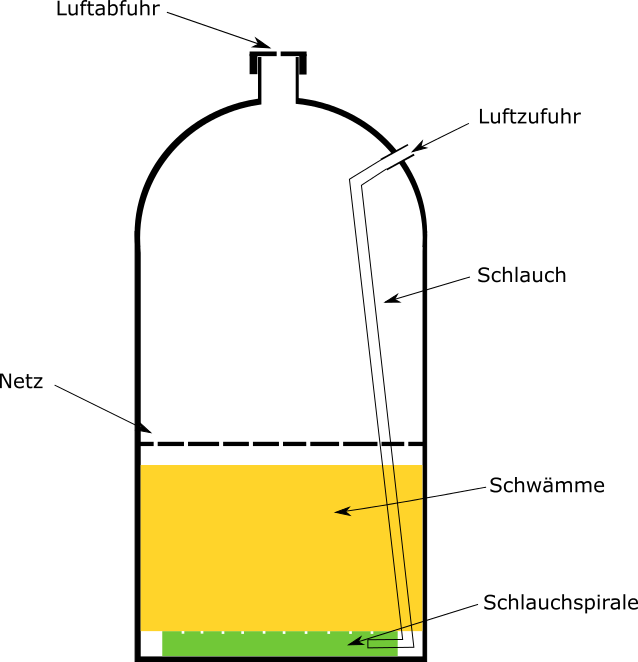
\includegraphics[scale=0.5]{Luftbefeuchter.png}
		\caption{Die Luft wird durch den den Schlauch in die Spirale geleitet und strömt dort aus feinen Löchern in die Schwämme. Die feinen Luftblasen nehmen Feuchtigkeit auf und die Luft strömt oben wieder aus dem Behälter.}
	\end{center}
\end{figure}

Beim Zusammenbau sahen die einzelnen Lage wie folgt aus:

\begin{figure}[h!]
	\begin{minipage}[hbt]{6cm}
		\centering
		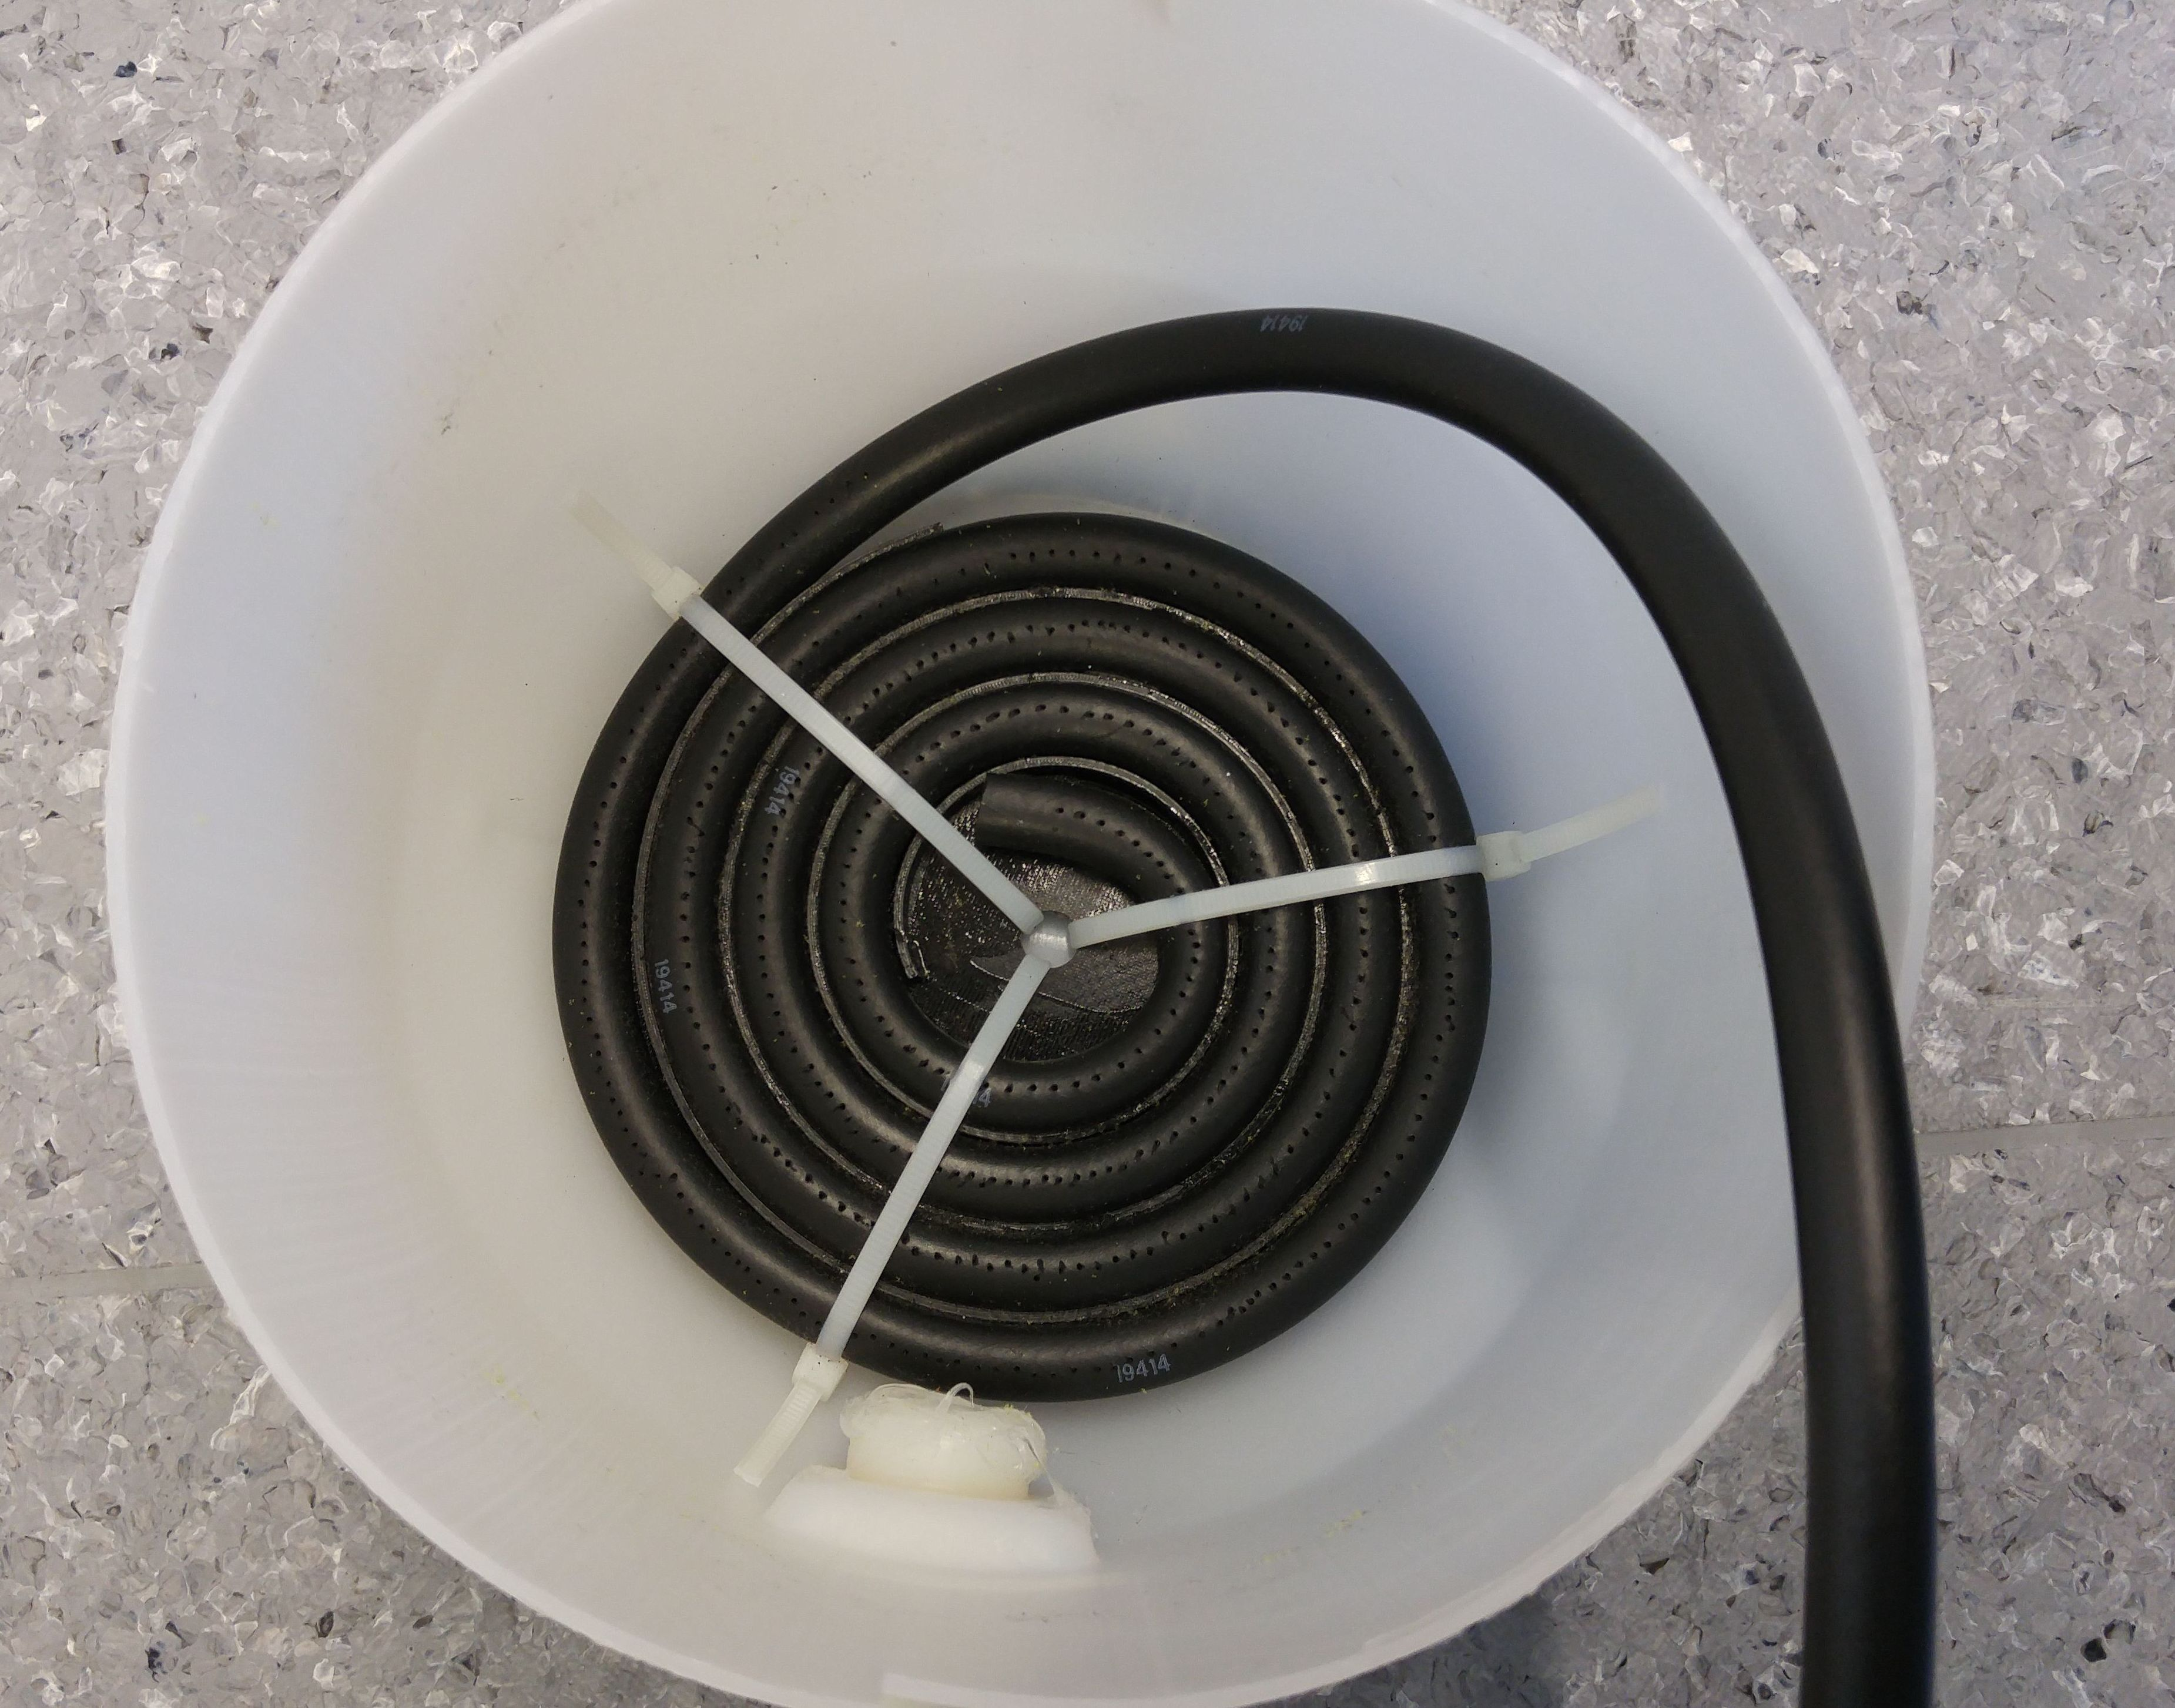
\includegraphics[width=6cm]{Luftbefeuchter_Spirale.jpg}
		\caption{Schlauchspirale durch die die Luft in die Schwämme geleitet wird}
	\end{minipage}
	\hfill
	\begin{minipage}[hbt]{6cm}
		\centering
		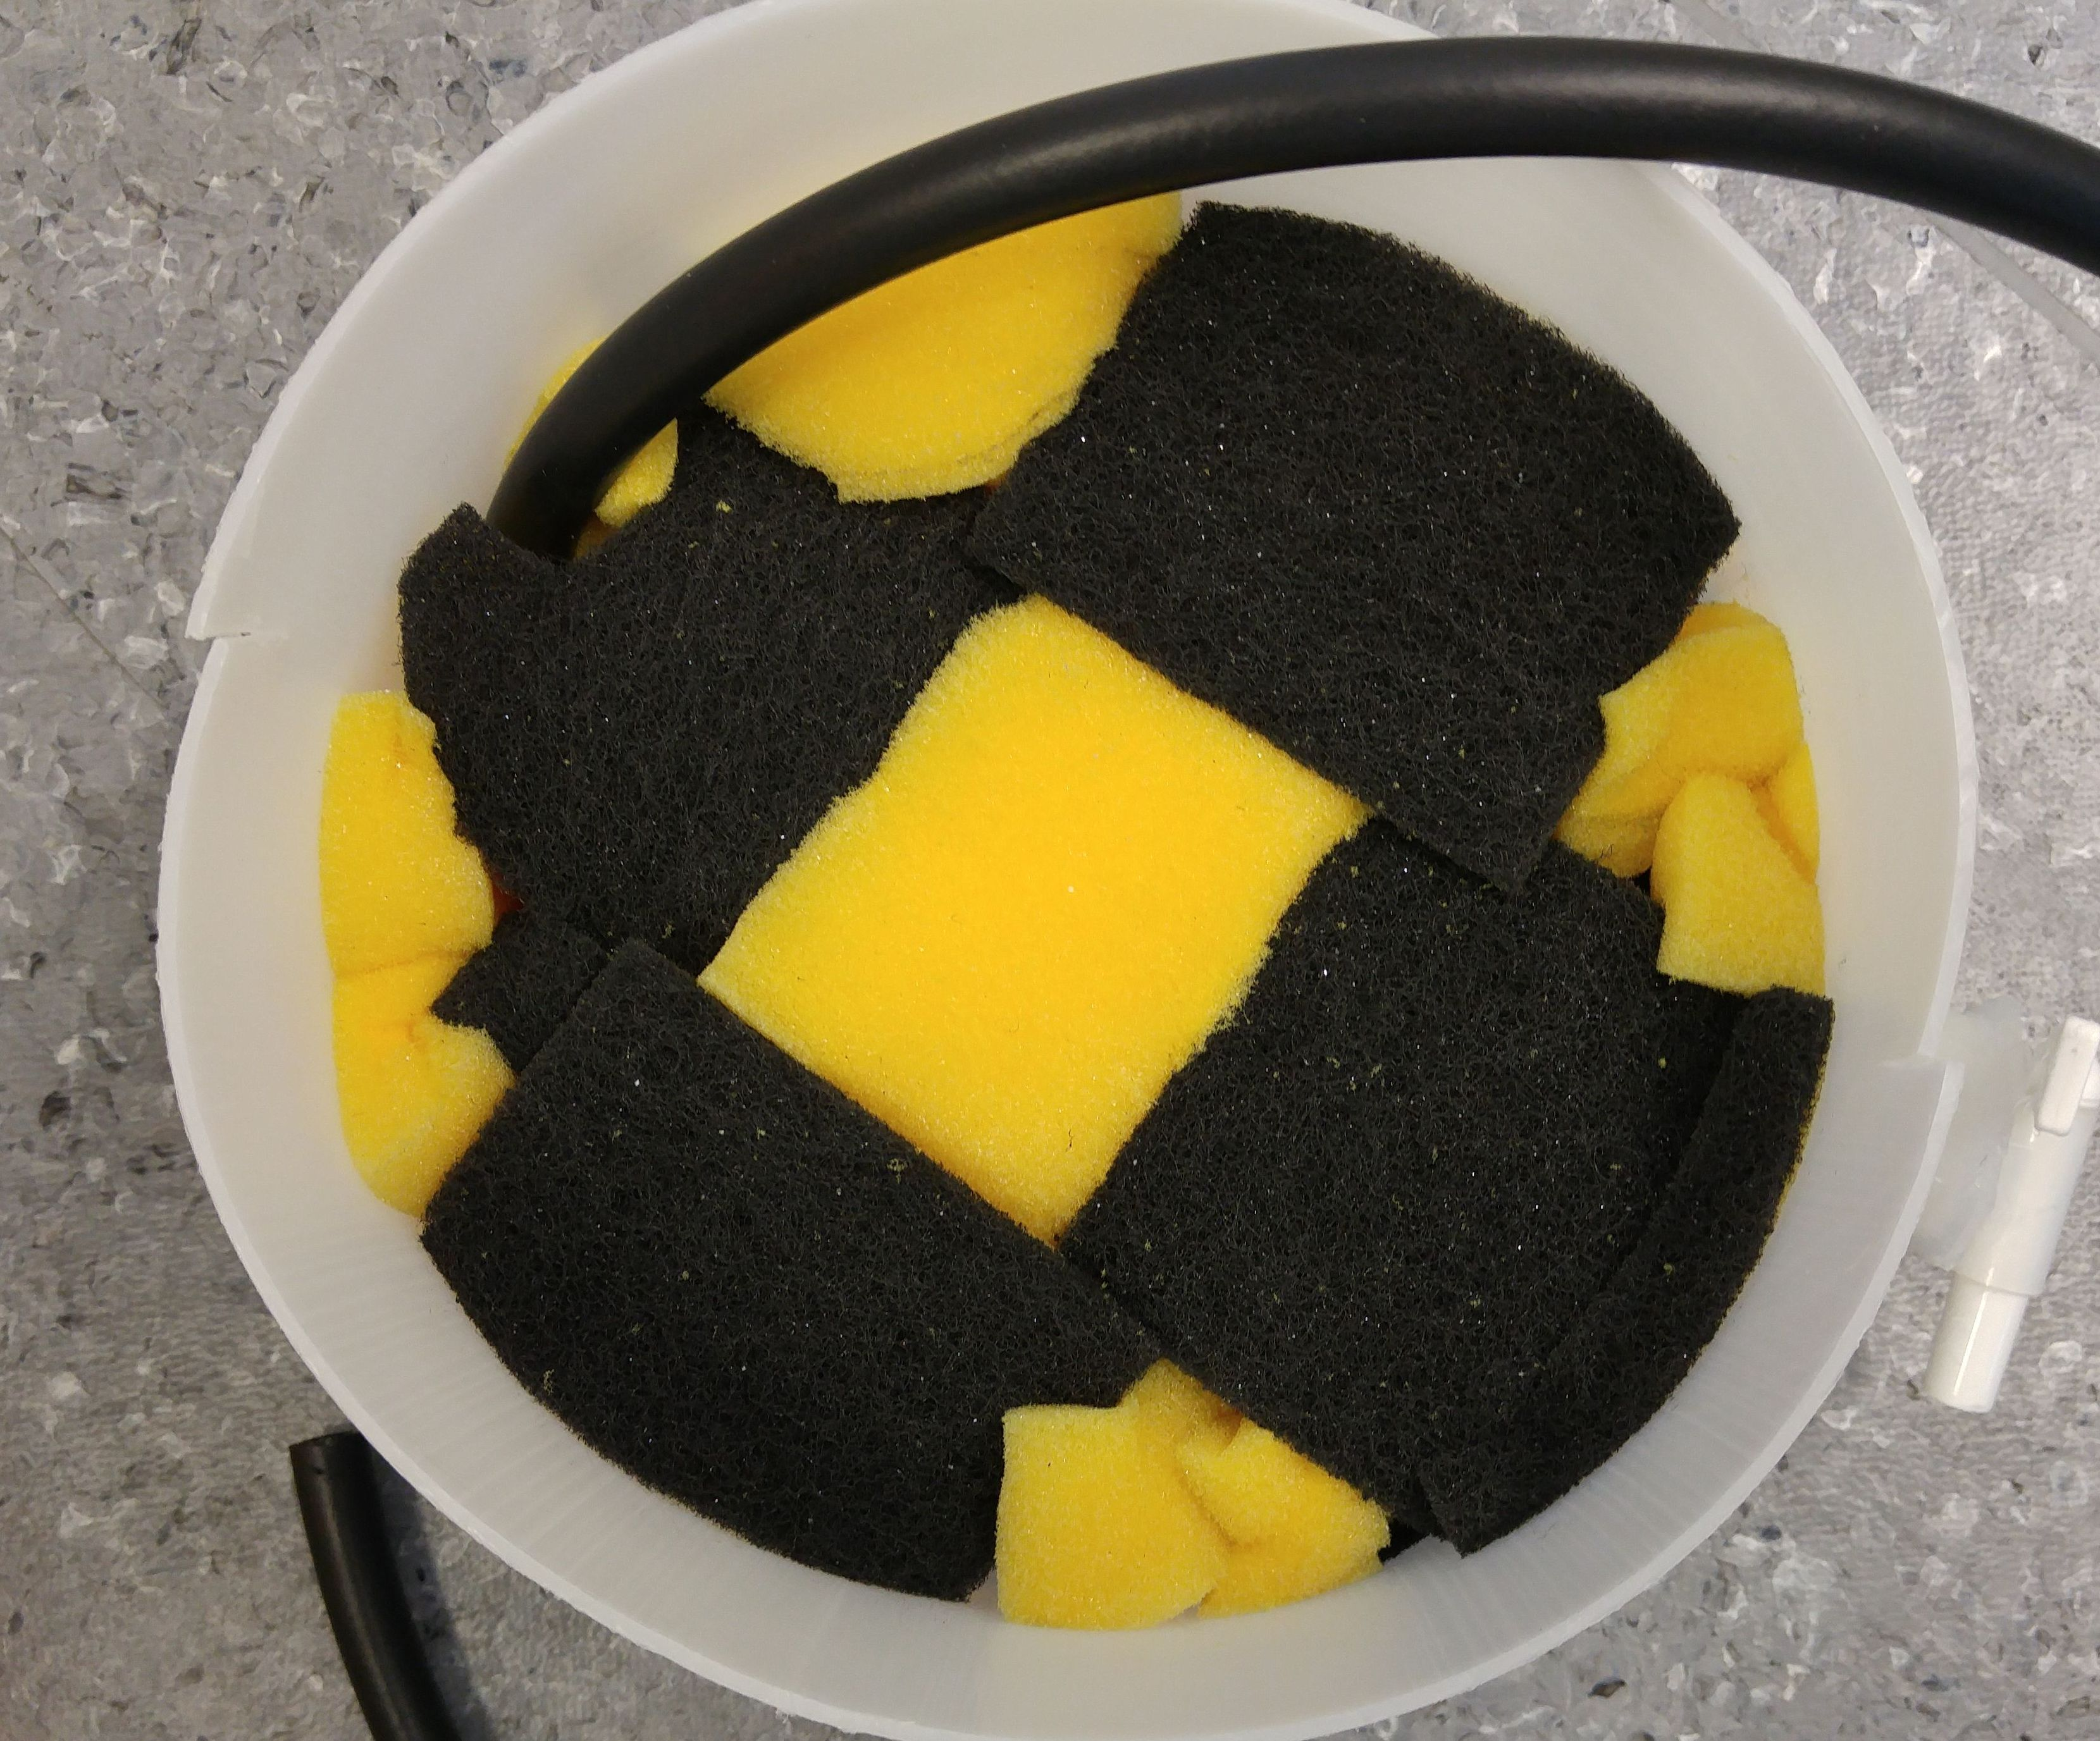
\includegraphics[width=6cm]{Luftbefeuchter_Schwaemme.jpg}
		\caption{Schwämme, die die kleinen Luftblasen erzeugen}
	\end{minipage}
\end{figure}

\begin{figure}[h!]
	\begin{minipage}[hbt]{6cm}
		\centering
		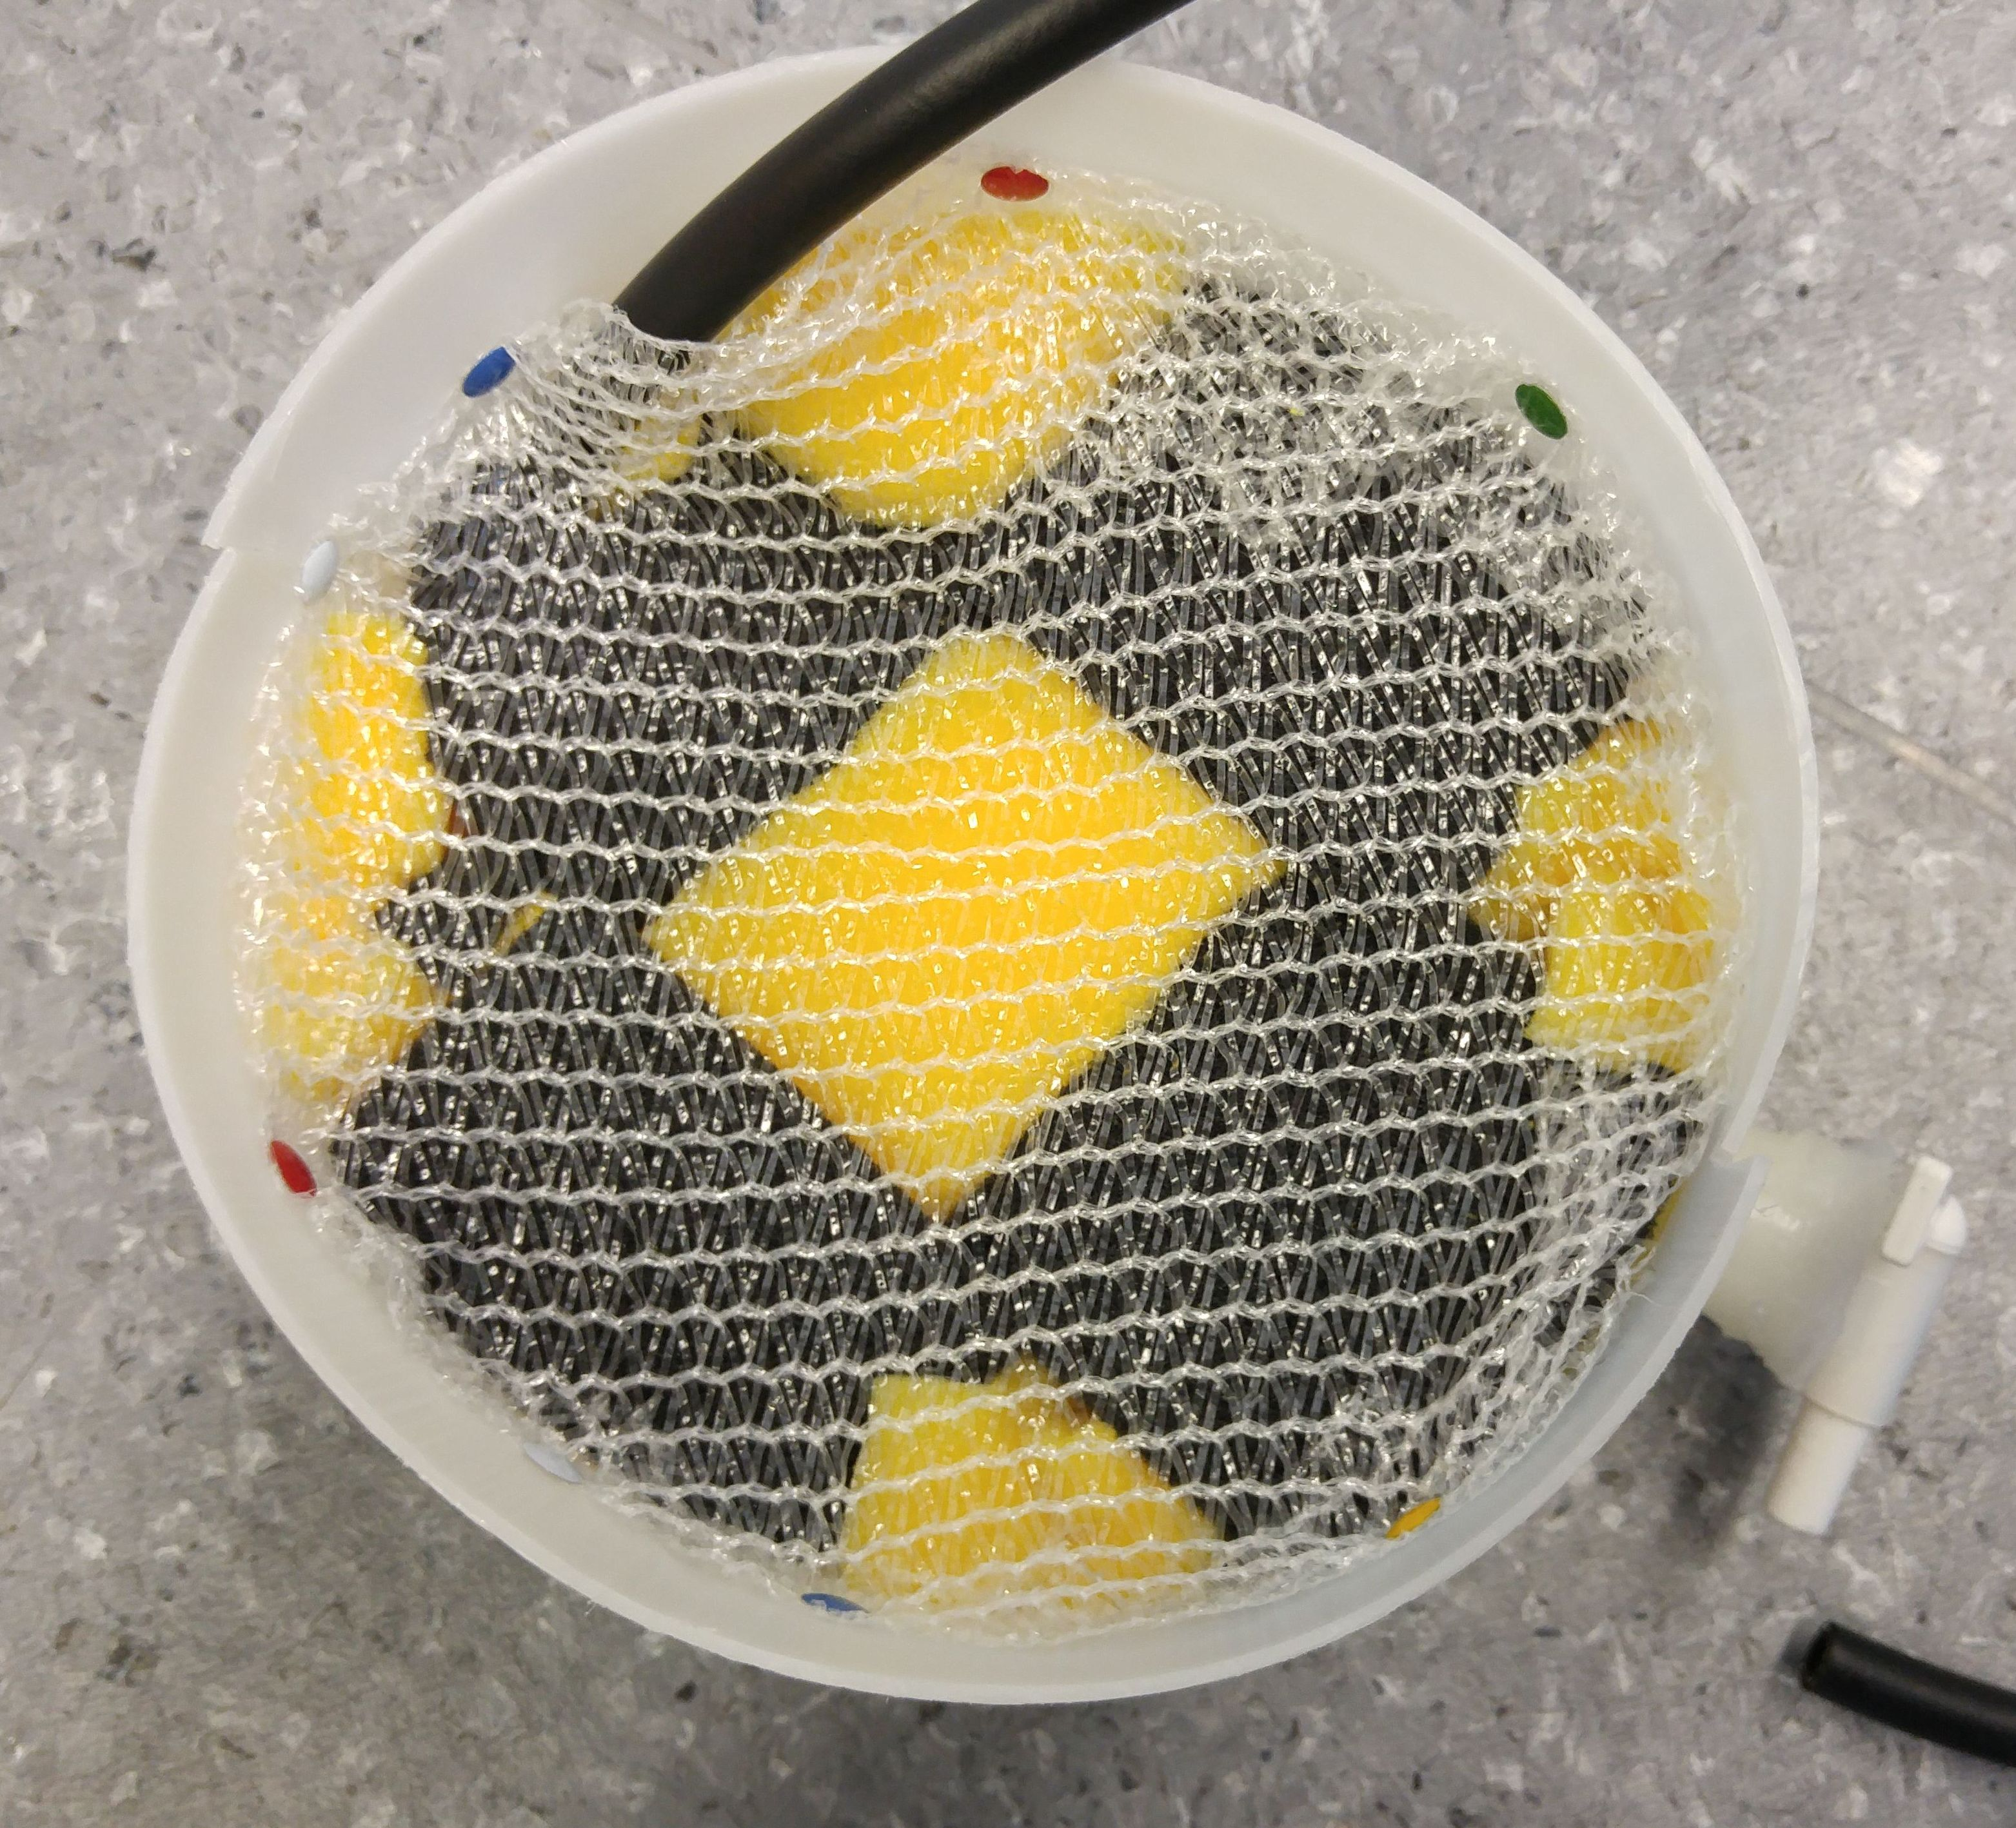
\includegraphics[width=6cm]{Luftbefeuchter_Netz.jpg}
		\caption{Netz, das die Schwämme an Position hält}
	\end{minipage}
	\hfill
	\begin{minipage}[hbt]{6cm}
		\centering
		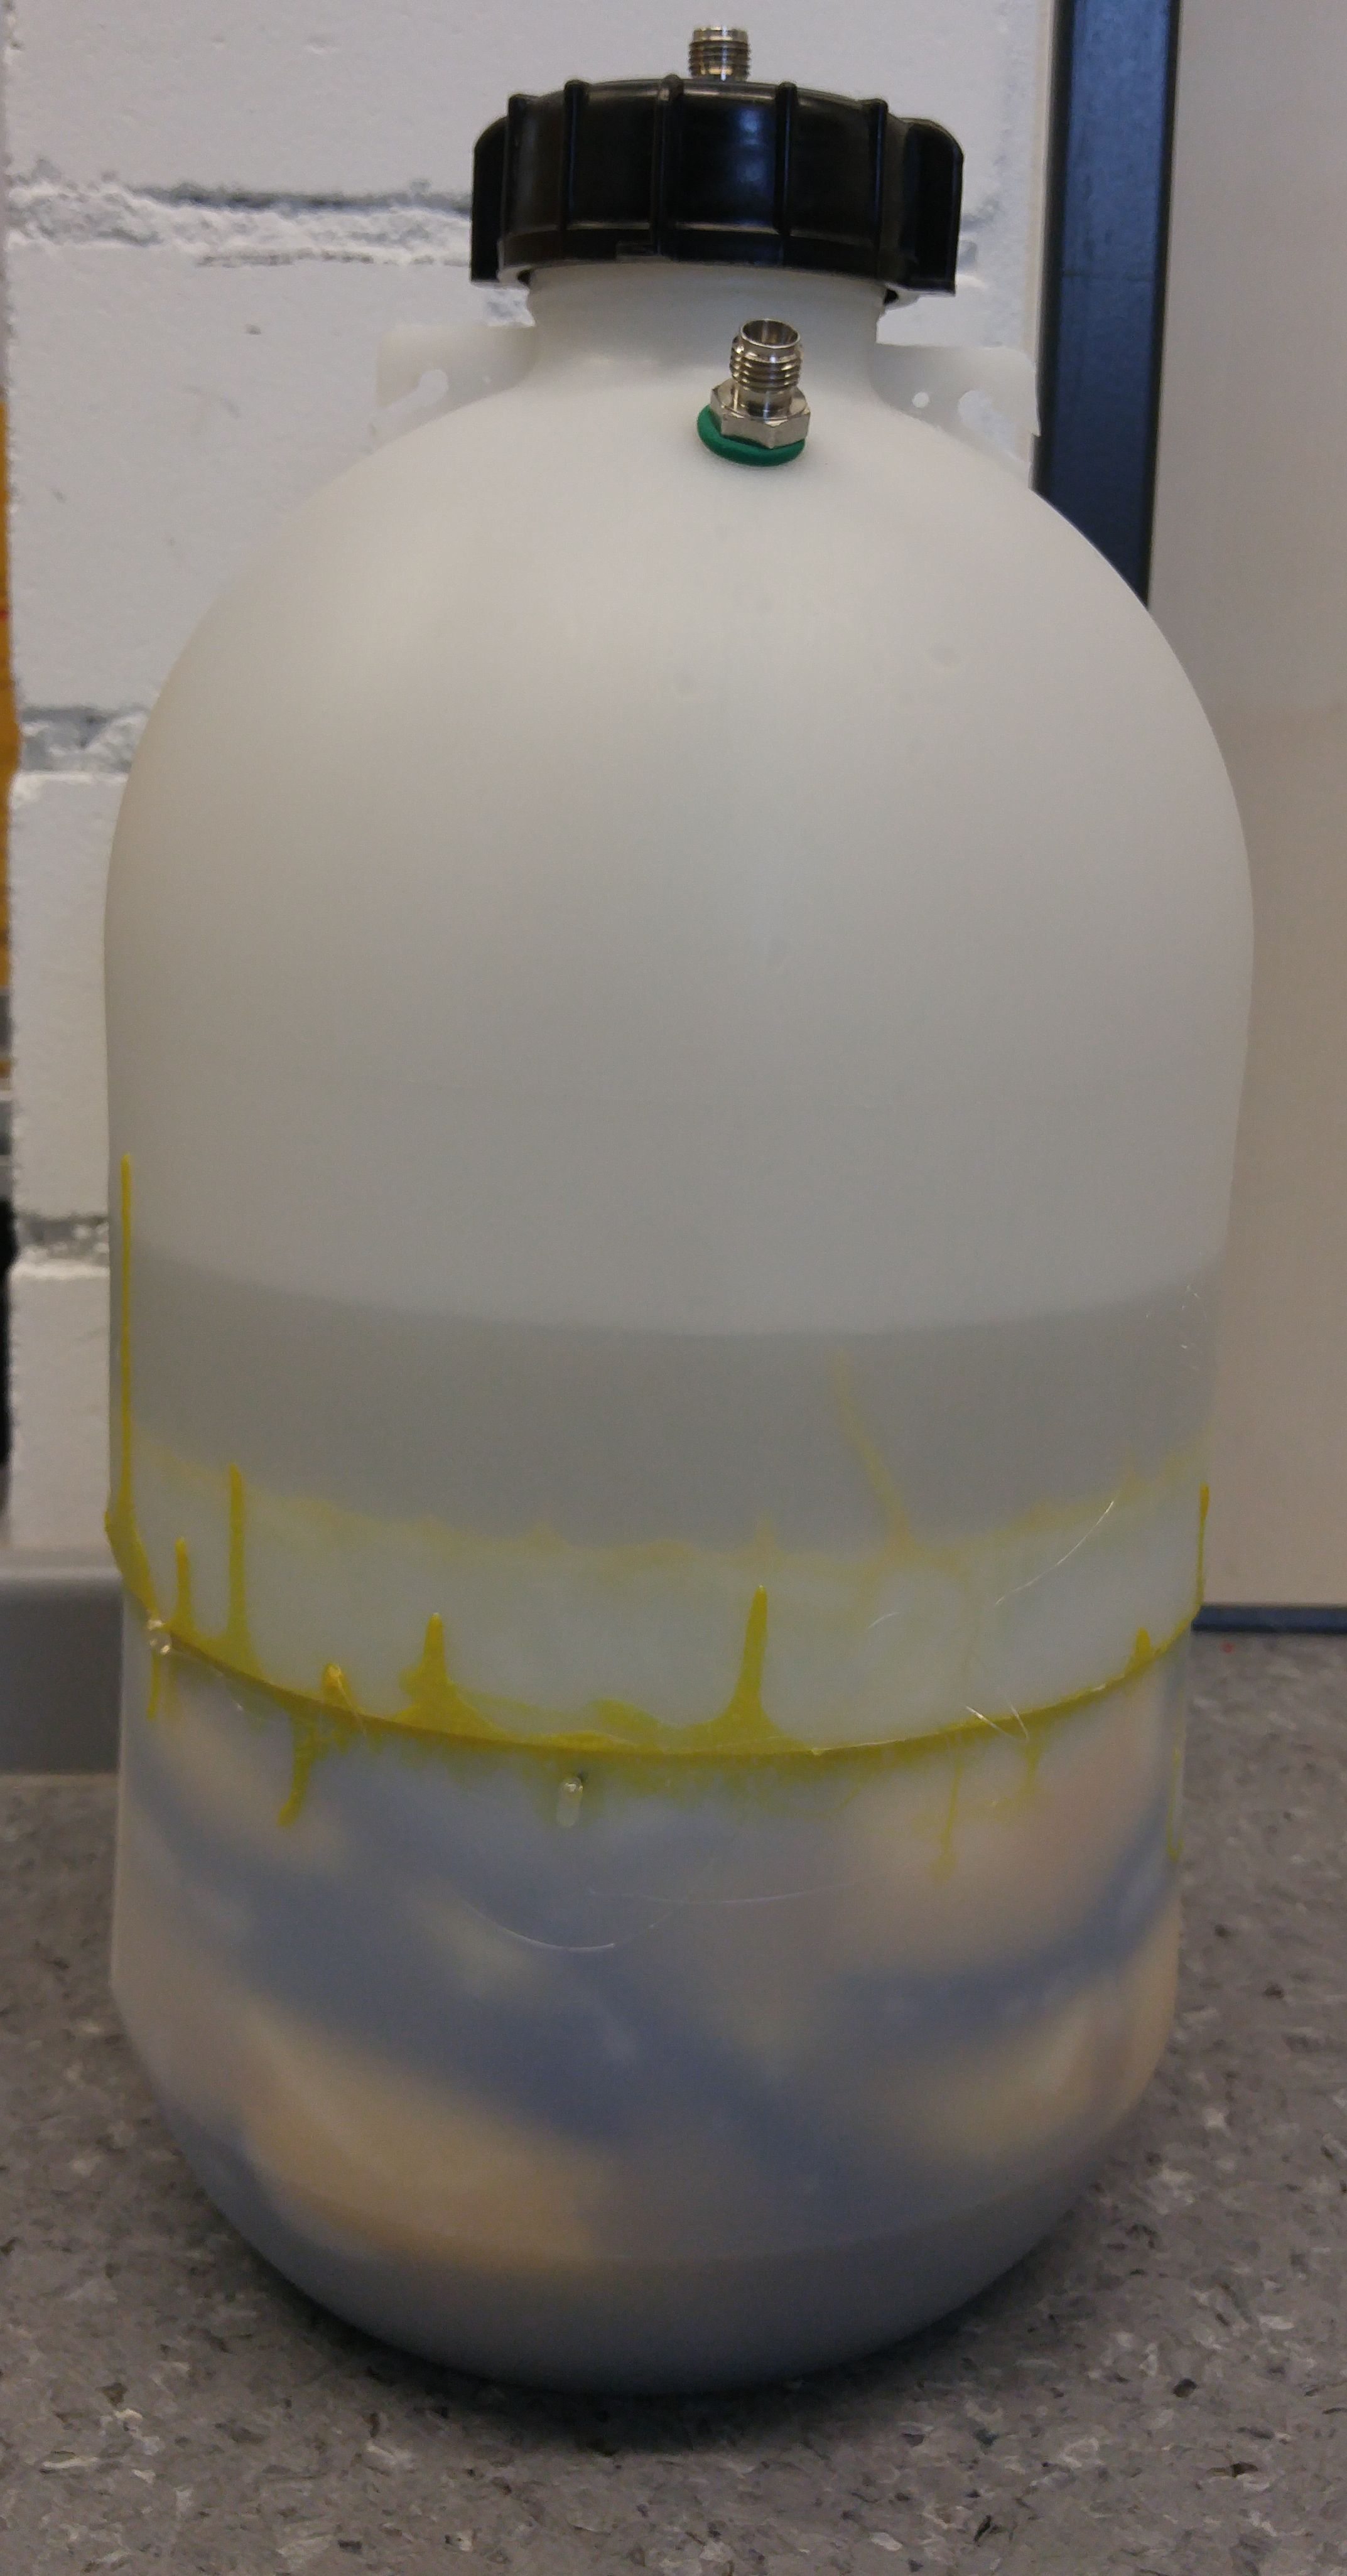
\includegraphics[width=6cm]{Luftbefeuchter_gesamt.jpg}
		\caption{Außenansicht in Betriebsbereitem Zustand}
	\end{minipage}
\end{figure}

\vspace{1cm}

Anschließend wurde in die obere Hälfte des Behälters eine Kombination aus einem Swagelok \SI{6}{mm} Rohrverbinder und einem Schlauchanschluss eingefügt. So kann man von außen ein Standard \SI{6}{mm} Stahlrohr anschließen und innen den Bunaschlauch für die Spirale. Die Lösung für die Luftabfuhr wurde ähnlich realisiert. Dazu wurde in den Verschluss wiederum ein \SI{6}{mm} Rohrverbinder eingefügt und der Verschluss auf der Innenseite mit einer Schicht Silikon ausgekleidet, sodass man ihn noch auf- und abdrehen kann um Wasser nachzufüllen, gleichzeitig aber die Luftdichtheit gewährleistet ist. Abschließend wurde auch der Luftbefeuchter auf einer Holzplatte befestigt, die auch dazu dient den Zu- und Ableitungsrohren möglichst wenig Bewegungsspielraum zu geben, sodass die Anschlüsse an den Befeuchter nicht belastet werden und es so nicht zu Undichtigkeiten kommt.

\newpage

\begin{figure}[h!]
	\begin{center}
		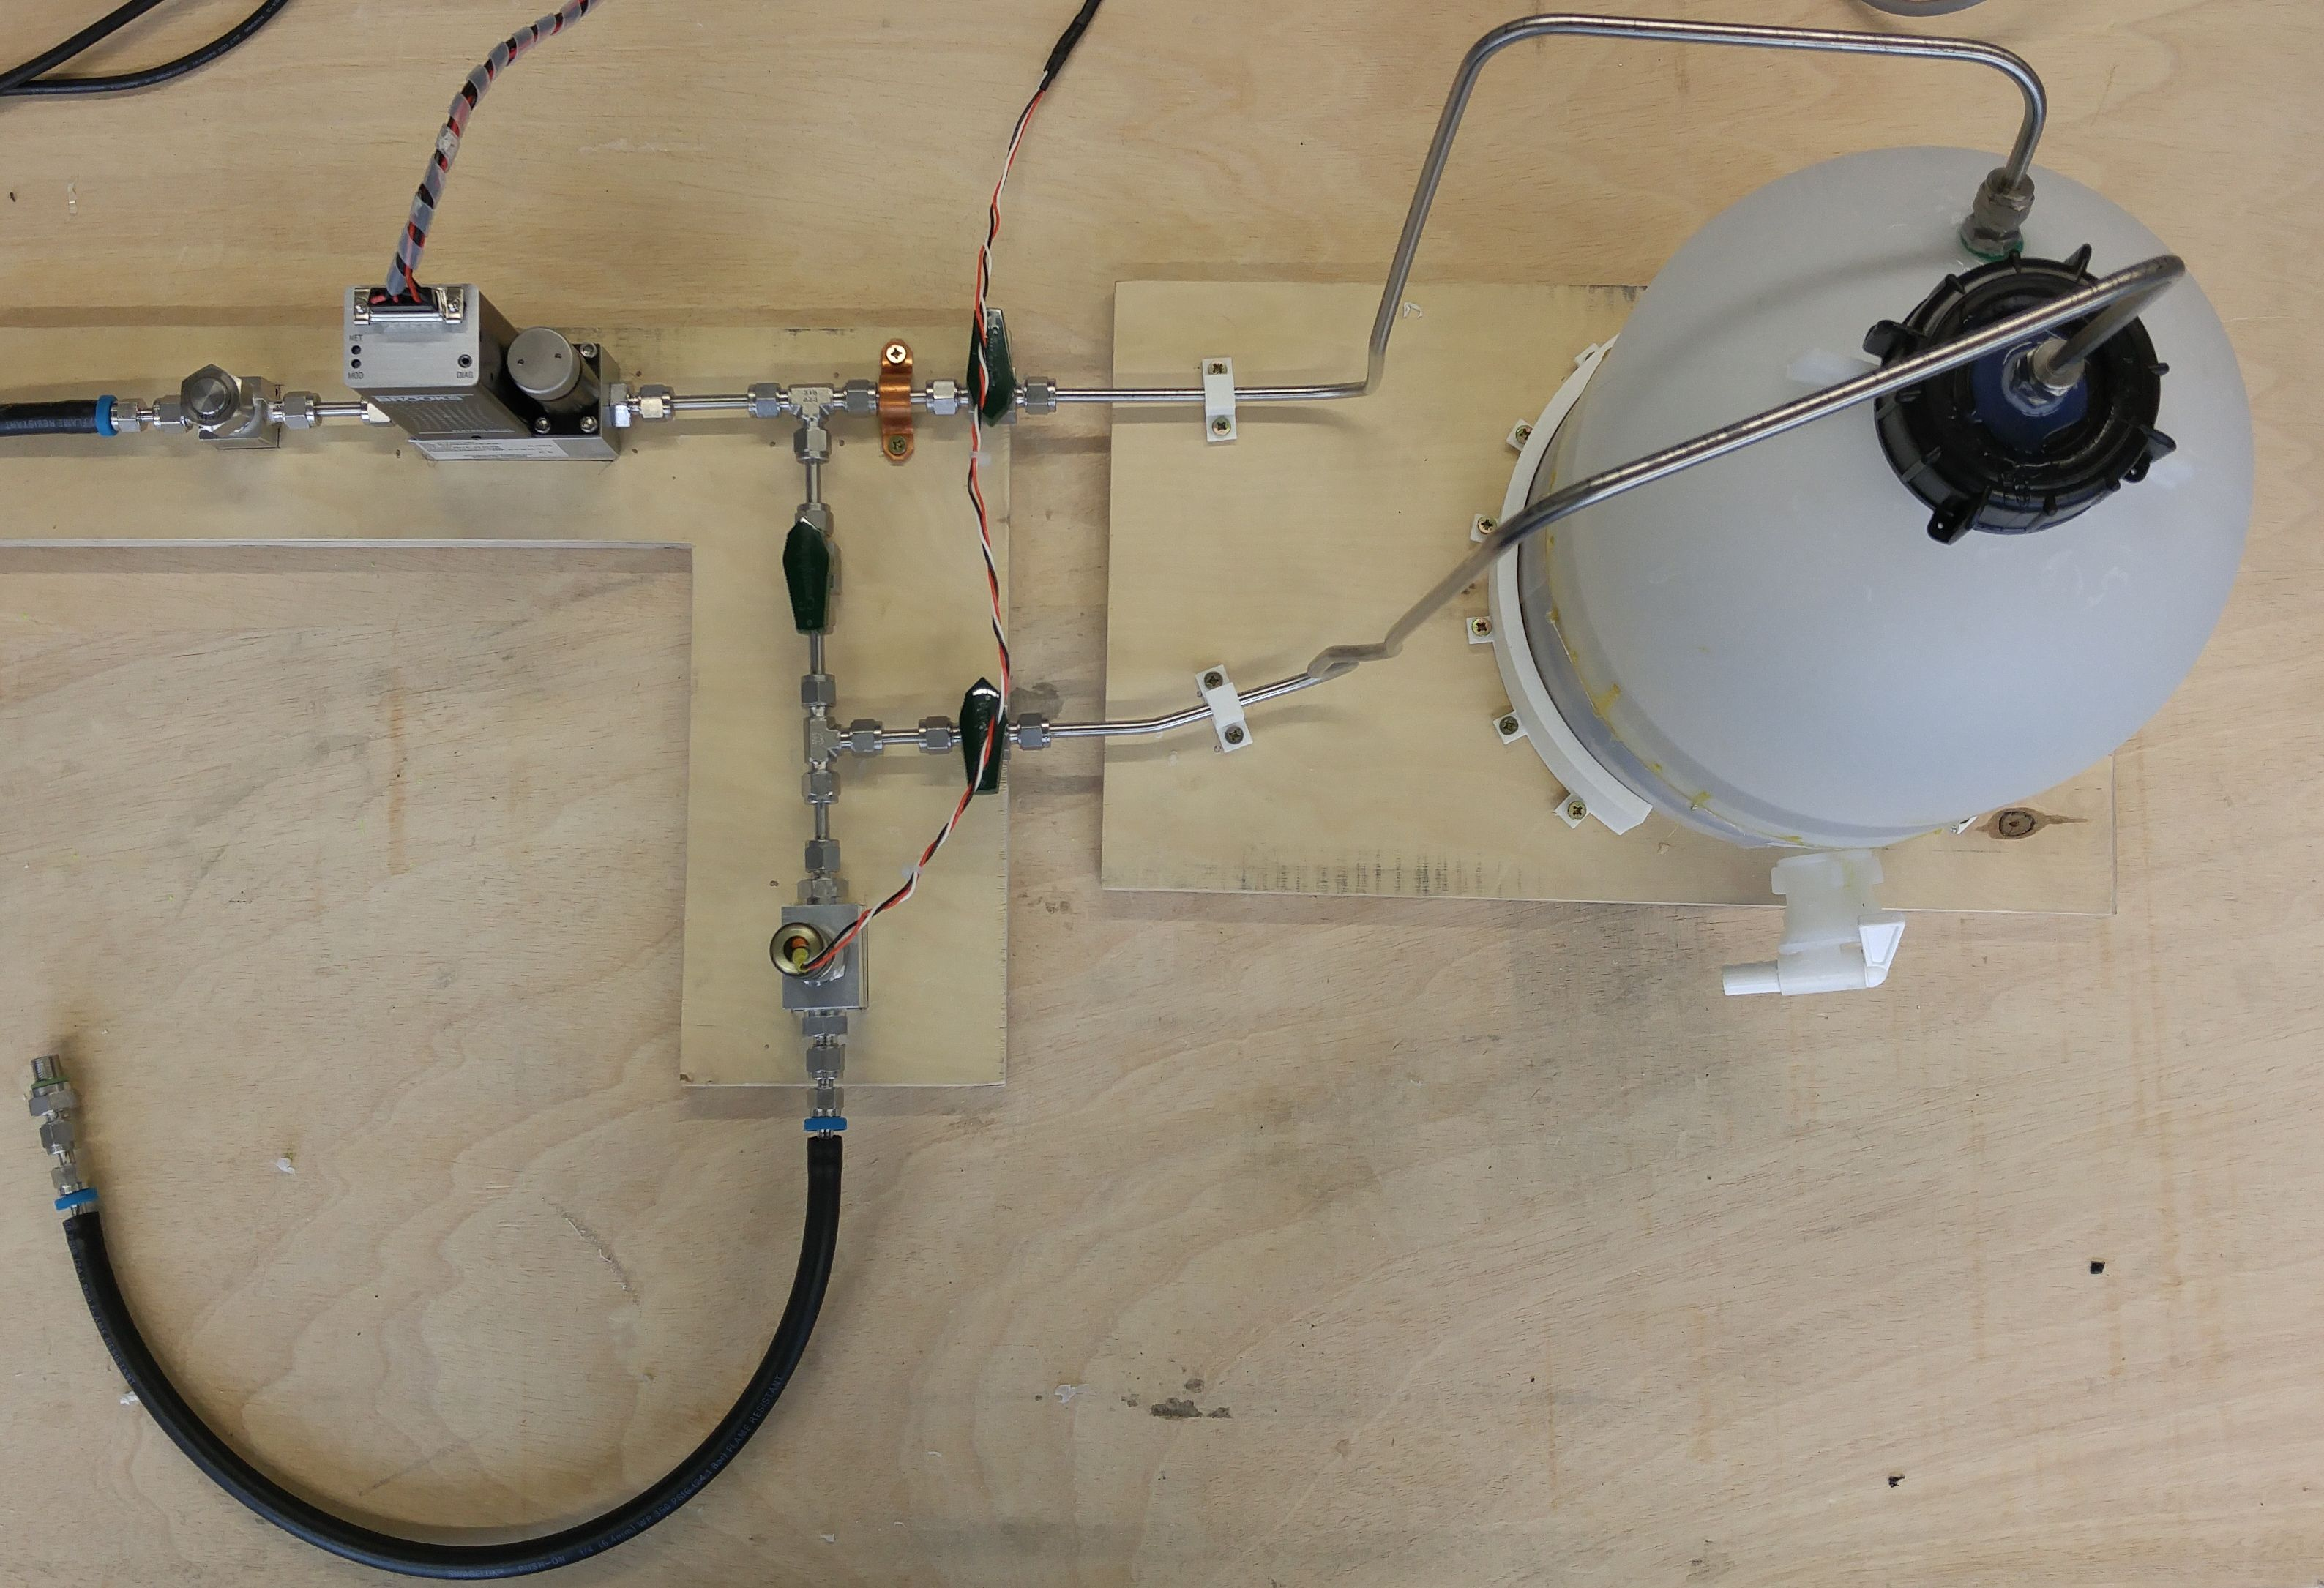
\includegraphics[scale=0.11]{Gassystem_montiert.jpg}
	\end{center}
\end{figure}


Im realen Betrieb wird die Luftfeuchtigkeit von \SI{75}{\%} nicht immer erreicht, stattdessen ist sie abhängig vom Luftstrom wie im Diagramm unten dargestellt.



\newpage


\section{AP4 - Wirbelbett}


\subsection{Allgemeine Anforderungen}

Da das bisherige Wirbelbett nicht flexibel genug konfigurierbar war, musste es neu konstruiert werden und dabei möglichst modular werden. Zum einen soll es möglich sein Probenröhrchen von \SI{5}{mm}, \SI{20}{mm}, \SI{30}{mm} und \SI{40}{mm} nutzen zu können. Weiterhin ist es erforderlich sowohl die Probenröhrchen als auch das Probenmaterial einfach und schnell wechseln zu können. Außerdem wurde gefordert, das aus dem Probenröhrchen austretende Partikel aufgefangen werden können. Des weiteren musste ein neuer Filter für den Übergang vom Anschlusszylinder zum Probenröhrchen gefunden werden. 
Eine weitere Anforderung bestand in der Integration eine Ionisators, sodass die durch das Probenröhrchen strömende Luft ionisiert werden kann. Die gesamte Konstruktion muss zudem in den Lichtstreuaufbau passen. \\




\begin{figure}[h]
	\begin{center}
		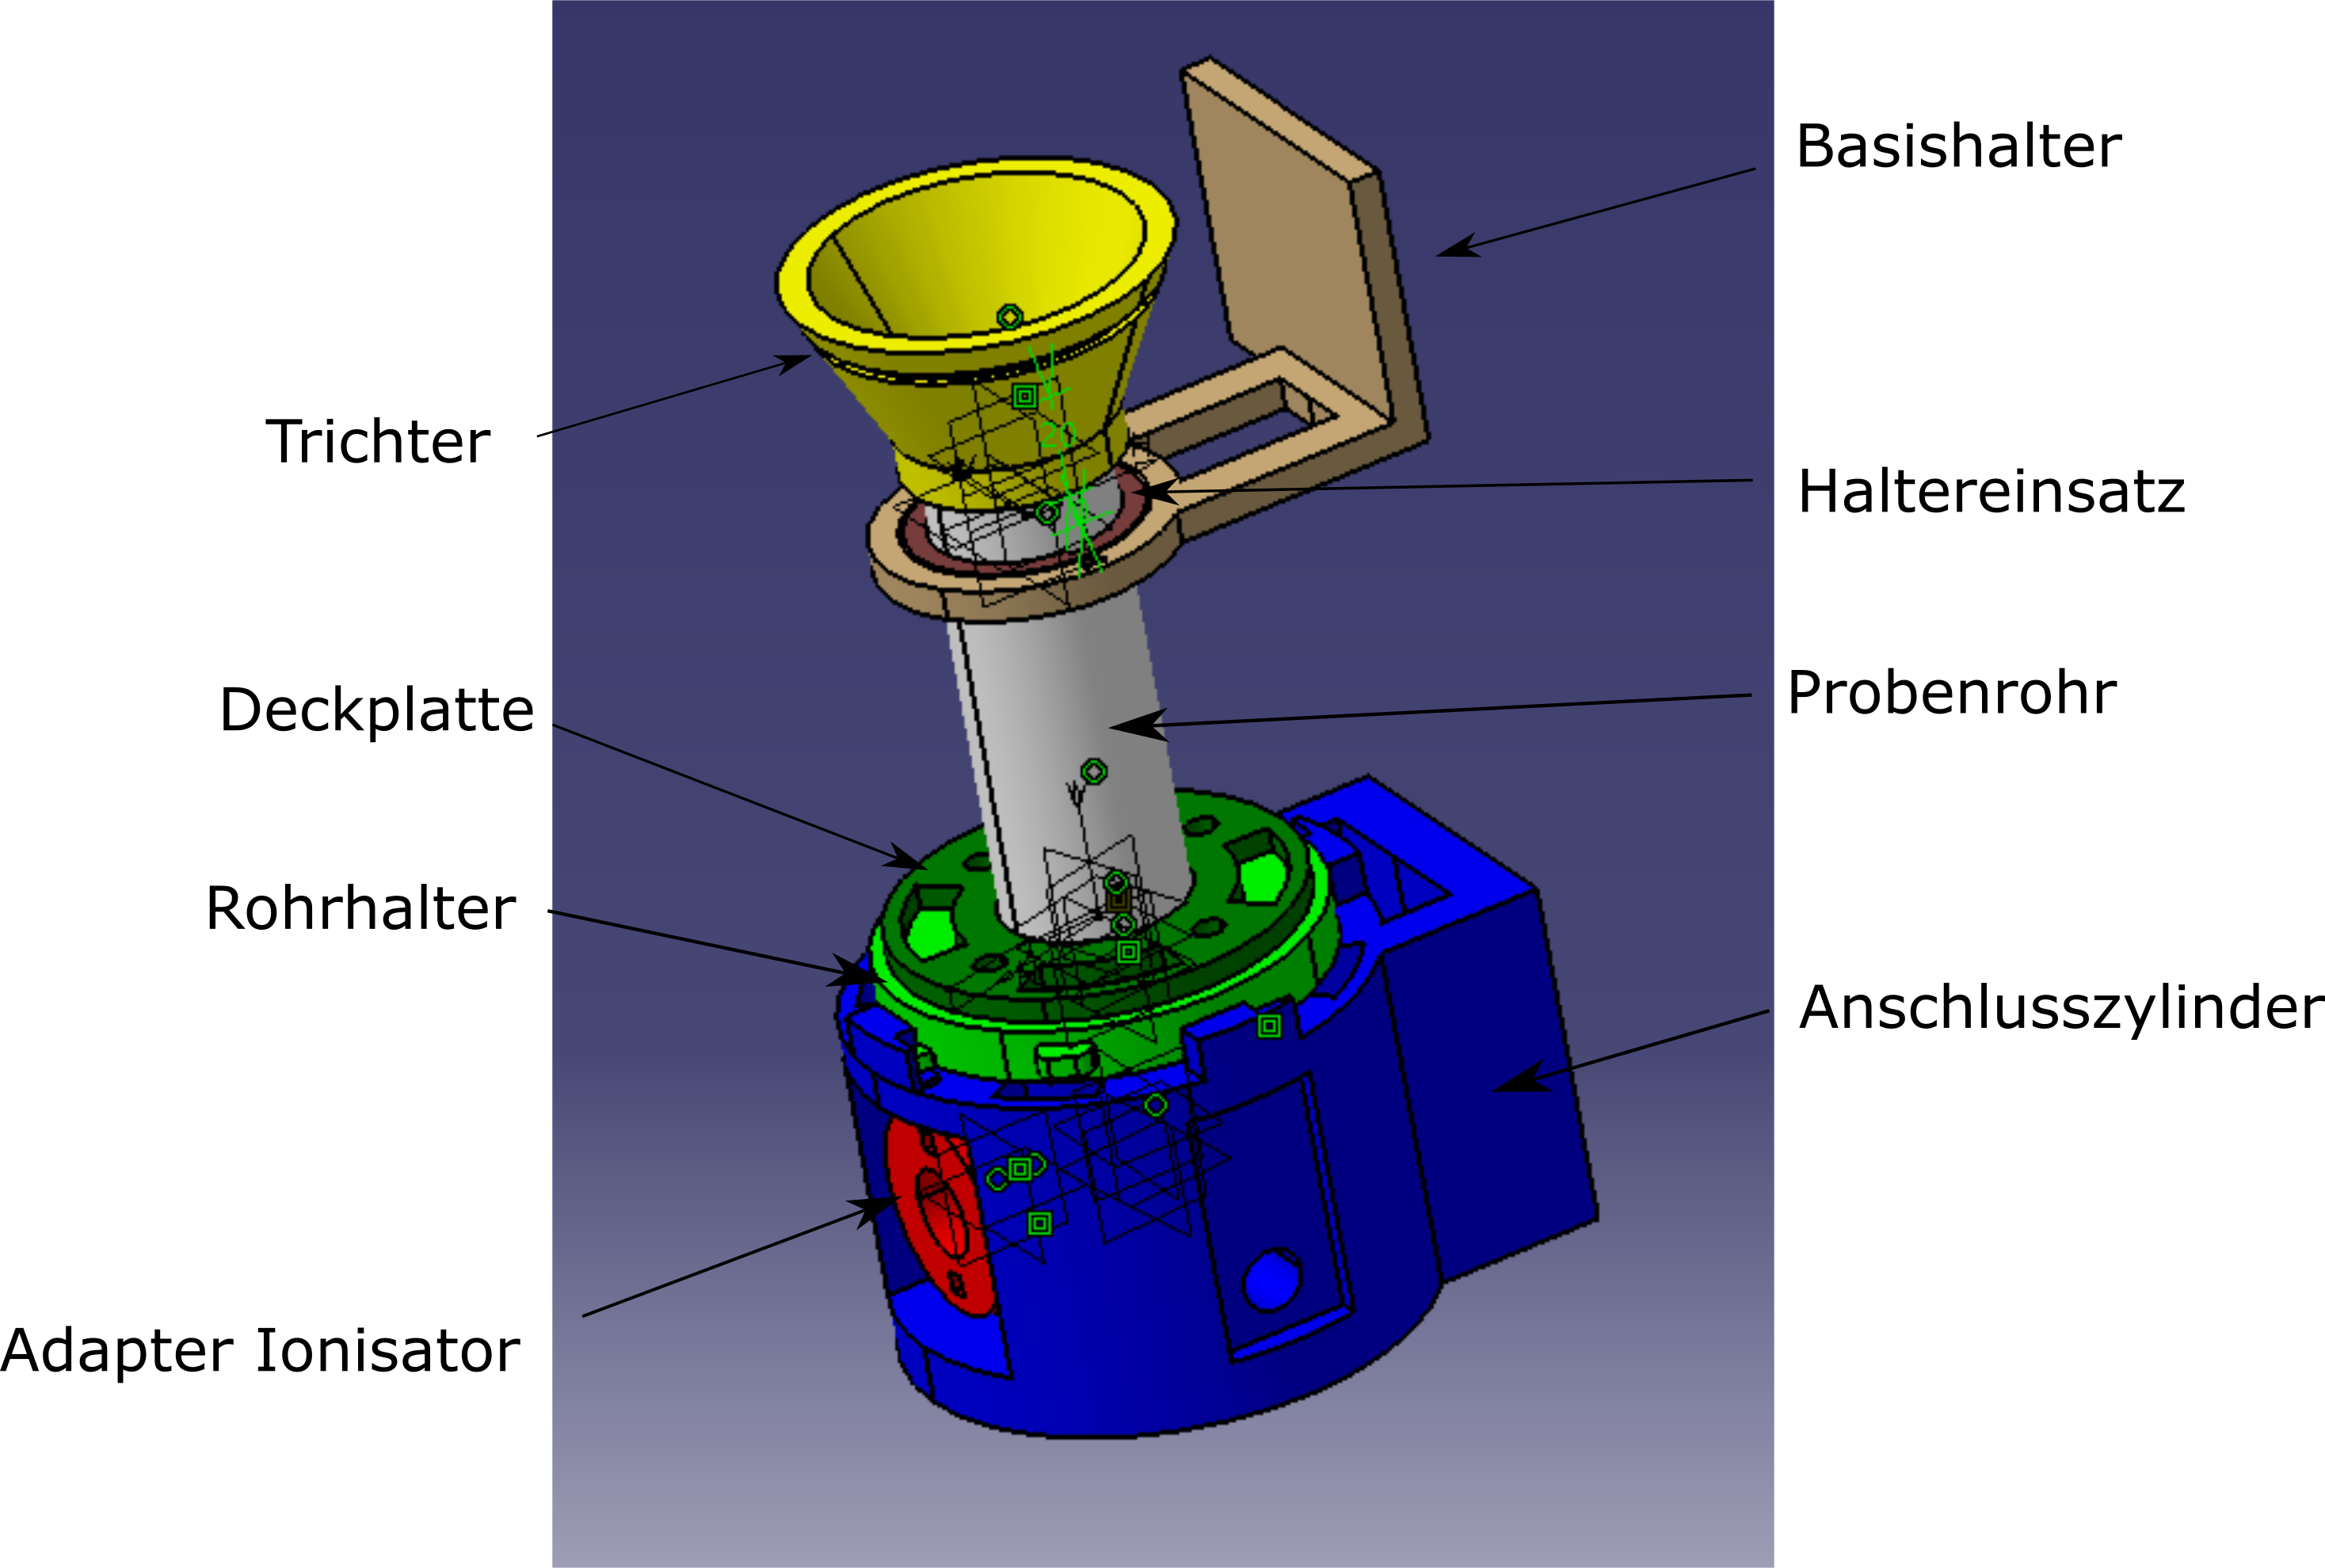
\includegraphics[scale=0.4]{Zusammenbau_fluides_Bett.png}
		\caption{Digitalmodell Wirbelbett}
	\end{center}
\end{figure}


Im folgenden werden die im Bild zu sehenden Bauteile in Abschnitten diskutiert, die sich mit der Methode zum auffangen des Granulats, dem Anschlusszylinder, dem Röhrchenhalter, der Halterung des Wirbelbetts und dem Filter beschäftigen.


\subsection{Methode zum Granulat auffangen}

\subsubsection{Anforderung}

Wie schon in der Einleitung beschrieben, hat ein granulares Medium mehrere Phasen gleichzeitig, von denen die oberste die Gasphase ist. Je nach Füllstand und Gasfluss des Messröhrchens kann es nun passieren, das einzelne Partikel oben aus dem Röhrchen hinausfliegen. Außerdem braucht es eine Absicherung gegen Fehlbedienung, sodass bei zu hohem Gasstrom kein Granulat aus dem Probenröchrchen austritt.

\subsubsection{Auswahl}

Ein in der Industrie übliches Produkt, um Luft von Partikeln zu säubern, ist der Fliehkraftabscheider oder Zyklon. Dieser basiert auf dem Prinzip, das die Luft immer weiter beschleunigt wird und die darin enthaltenen Partikel an die Wand gedrückt werden und schließlich nach unten raus fallen. \\


\begin{figure}[h]
	\begin{center}
		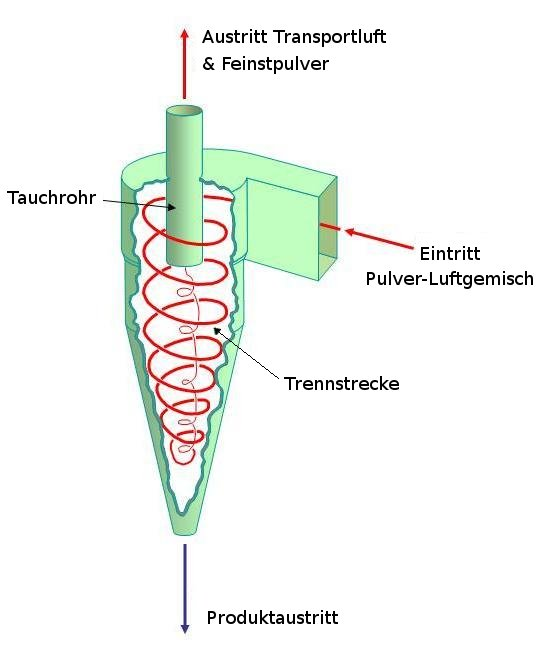
\includegraphics[scale=0.5]{Umsetzung_Fliehkraftabscheider.jpg}
		\caption{Funktionsweise eines klassischen Fliehkraftabscheiders: Quelle Wikipedia}
	\end{center}
\end{figure}



Das Problem bei diesem Bauteil besteht darin, das die kommerziell erhältlichen Versionen sehr teuer sind und zudem zu groß für unserem Aufbau passen. \\
Weiterhin wäre ein erheblicher Konstruktionsaufwand nötig, um einen eigenen Zyklon zu bauen, da die Luft in unserem Versuch von unten kommt, der Zyklon sie aber von der Seite braucht. \\
Eine Alternative dazu ist ein Trichter, der den Querschnitt aufweitet und so den Gasstrom verlangsamt. Aus Kosten und den oben beschriebenen Konstruktionsproblemen wurde entschieden einen Trichter zu entwerfen.



\subsubsection{Umsetzung}

Um den Gasstrom zu verlangsamen und gleichzeitig das Einfüllen des Granulats zu erleichtern, wurde jeweils ein Trichter konstruiert, der passgenau mit dem Innendurchmesser jedes Probenröhrchens abschließt und zudem den Querschnitt verdoppelt. \\
Wie man anhand der Formel $v_a = \frac{Q}{A}$ \cite{Grollius2012} sehen kann, ist die Geschwindigkeit des Gasstrom direkt proportional zum Querschnitt des Rohrs. Wenn man also den Querschnitt verdoppelt, dann viertelt man die Geschwindigkeit des Gasstroms. Dies wurde für jeden Durchmesser gemacht. Man könnte zwar bei gleicher Höhe auch die Querschnitte unter \SI{40}{mm} auf \SI{80}{mm} aufweiten, allerdings bringt das stömungstechnisch nicht viel, da sich der Luftstrom nicht so schnell so stark aufweiten kann. \\
Zudem wurde ein abnehmbarer Filter oben auf den Trichter gespannt, um einen rudimentären Schutz gegen austretende Partikel bei Fehlbedienung zu gewährleisten.

\begin{figure}[h]
	\begin{center}
		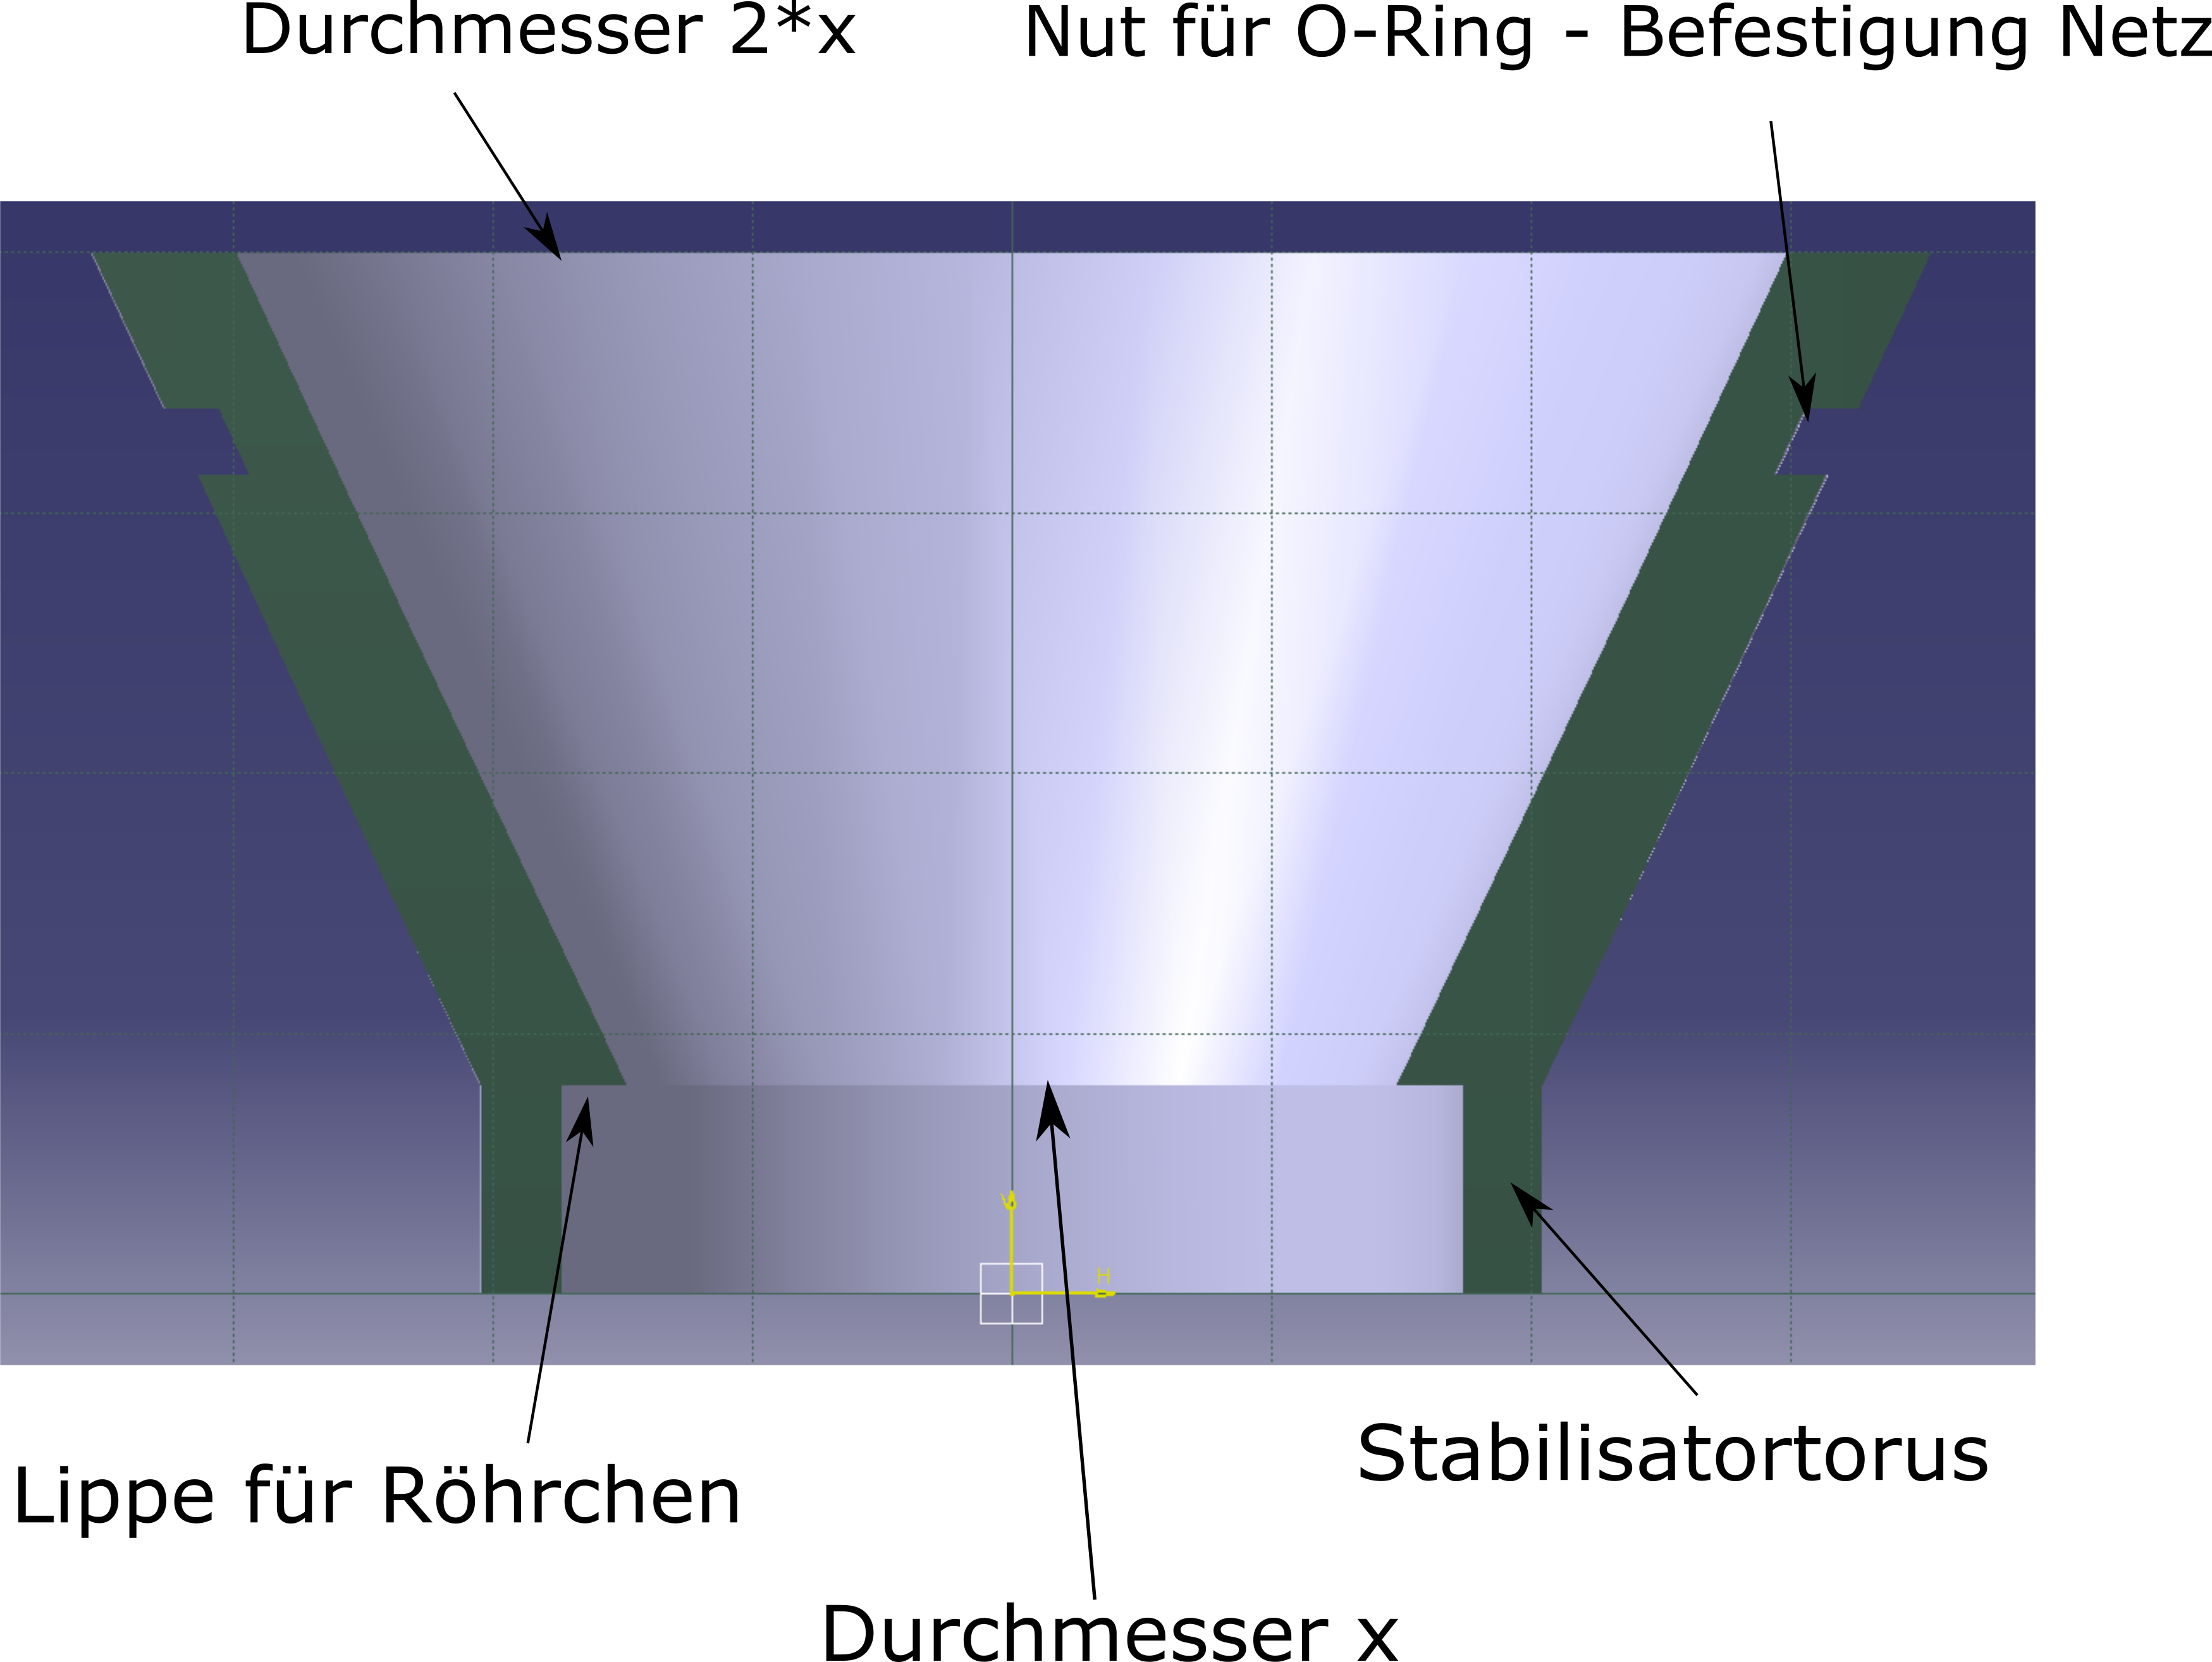
\includegraphics[scale=0.5]{Schnitt_Trichter.png}
	\end{center}
\end{figure}

\newpage

\subsection{Anschlusszylinder}

\subsubsection{Anforderungen}

Das Ziel bei diesem Zylinder war den Anschluss an das Gassystem zu haben und eine Halterung für die verschieden großen Röhrchen zu haben, die einen schnellen Wechsel gewährleistet. Zudem sollte gewährleistet werden, das ein Ionisator in den Luftstrom eingebracht werden kann.


\subsubsection{Umsetzung}

Der Kern des Anschlusszylinders ist die $\SI{40}{mm}$ breite Röhre, damit Röhrchendurchmesser bis $\SI{40}{mm}$ mit einem laminaren Gasstrom versorgt werden können. Belegen lässt sich der laminare Gasstrom durch die Reynoldszahl. Dazu wird zunächst die Gasgeschwindigkeit $v_{Gas}$ berechnet:

\begin{align*}
v_{Gas} = \frac{Q}{A}
\end{align*}
Dabei ist $Q$ die Gasmenge in $m^3$, die pro Sekunde durch das Röhrchen strömt und $A$ die Querschnittsfläche des Röhrchens in $m^2$. Mit der Gasgeschwindigkeit berechnet man dann die Reynoldszahl:
\begin{align*}
Re = \frac{v_{Gas} \cdot d}{\nu}
\end{align*} 
Dabei ist $d$ der innere Durchmesser des Anschlusszylinders und $\nu$ die kinetische Viskosität der Luft. Für den maximalen Gasstrom von $\SI{3}{m^3/h}$, lautet die Rechnung wie folgt:

\begin{align*}
v_{Gas} &= \frac{\frac{\SI{3}{m^3}}{\SI{3600}{s}}}{\pi \cdot \SI{0,02}{m}^2} = \SI{0,66}{m/s} 
\intertext{Damit ergibt die sich Reynoldszahl zu:}
Re &= \frac{\SI{0,66}{m/s} \cdot \SI{0,04}{m}}{ \nu\footnotemark[1]} = 1724,36
\end{align*}

\footnotetext[1]{kinematische Viskosität von Luft = $\SI{15,31}{m^2/s}$ bei Normaldruck und \SI{20}{^\circ C}}

Die Reynoldszahl ist kleiner als 2300, damit ist der Gasstrom laminar. \\
Auf der Oberseite befindet sich eine Nut in die der O-Ring zum Abdichten der Verbindung Anschlusszylinder-Röhrchenhalter eingelegt wird. Damit diese Verbindung dicht ist, befindet sich auf der Oberseite zudem ein Arretierungsmechanismus in den der Röhrchenhalter eingedreht wird. Zudem garantiert dieser Mechanismus ein einfaches und schnelles lösen der Komponenten. Um das Dichtverhalten zwischen Plastik und O-Ring zu verbessern wurde Silikon mit dem O-Ring verbunden. Dies geschieht indem man Silikon (Elastosil E43, Wacker) in beide Nute streicht den O-Ring einlegt und den Mechanismus zwei Tage lang arretiert lässt. Nach dem Aushärten sind O-Ring und Silikon verbunden und zeigen nun optimales Dichtverhalten. 
Zum arretieren muss eine Kraft von \SI{60}{N} auf die Silikon-Gummi Dichtung ausgeübt werden. Bei Arretierung wird diese Kraft an acht Punkten gehalten, jeder Punkt hält also \SI{7,5}{N}. In Versuchen stellte sich heraus, das jeder dieser Punkte erst bei einer Krafteinwirkung von \SI{75}{N} anfängt nachzugeben. Die Festigkeit im Arbeitsbereich ist mit einem Sicherheitsfaktor von ca 10 garantiert. Die Messmethoden zur Feststellung dieser Werte sind wie folgt: \hfill \\
Der Anschlusszylinder wird mit Röhrchenhalter im arretierten Zustand unter die das Kraftmessgerät (Ametek Chatillion DFS-025) gefahren, anschließend wir die Arretierung gelöst und der vom Messgerät angezeigte Wert, ist die nötige Kraft, die zur Arretierung benötigt wird. 

\begin{figure}[h]
	\begin{center}
		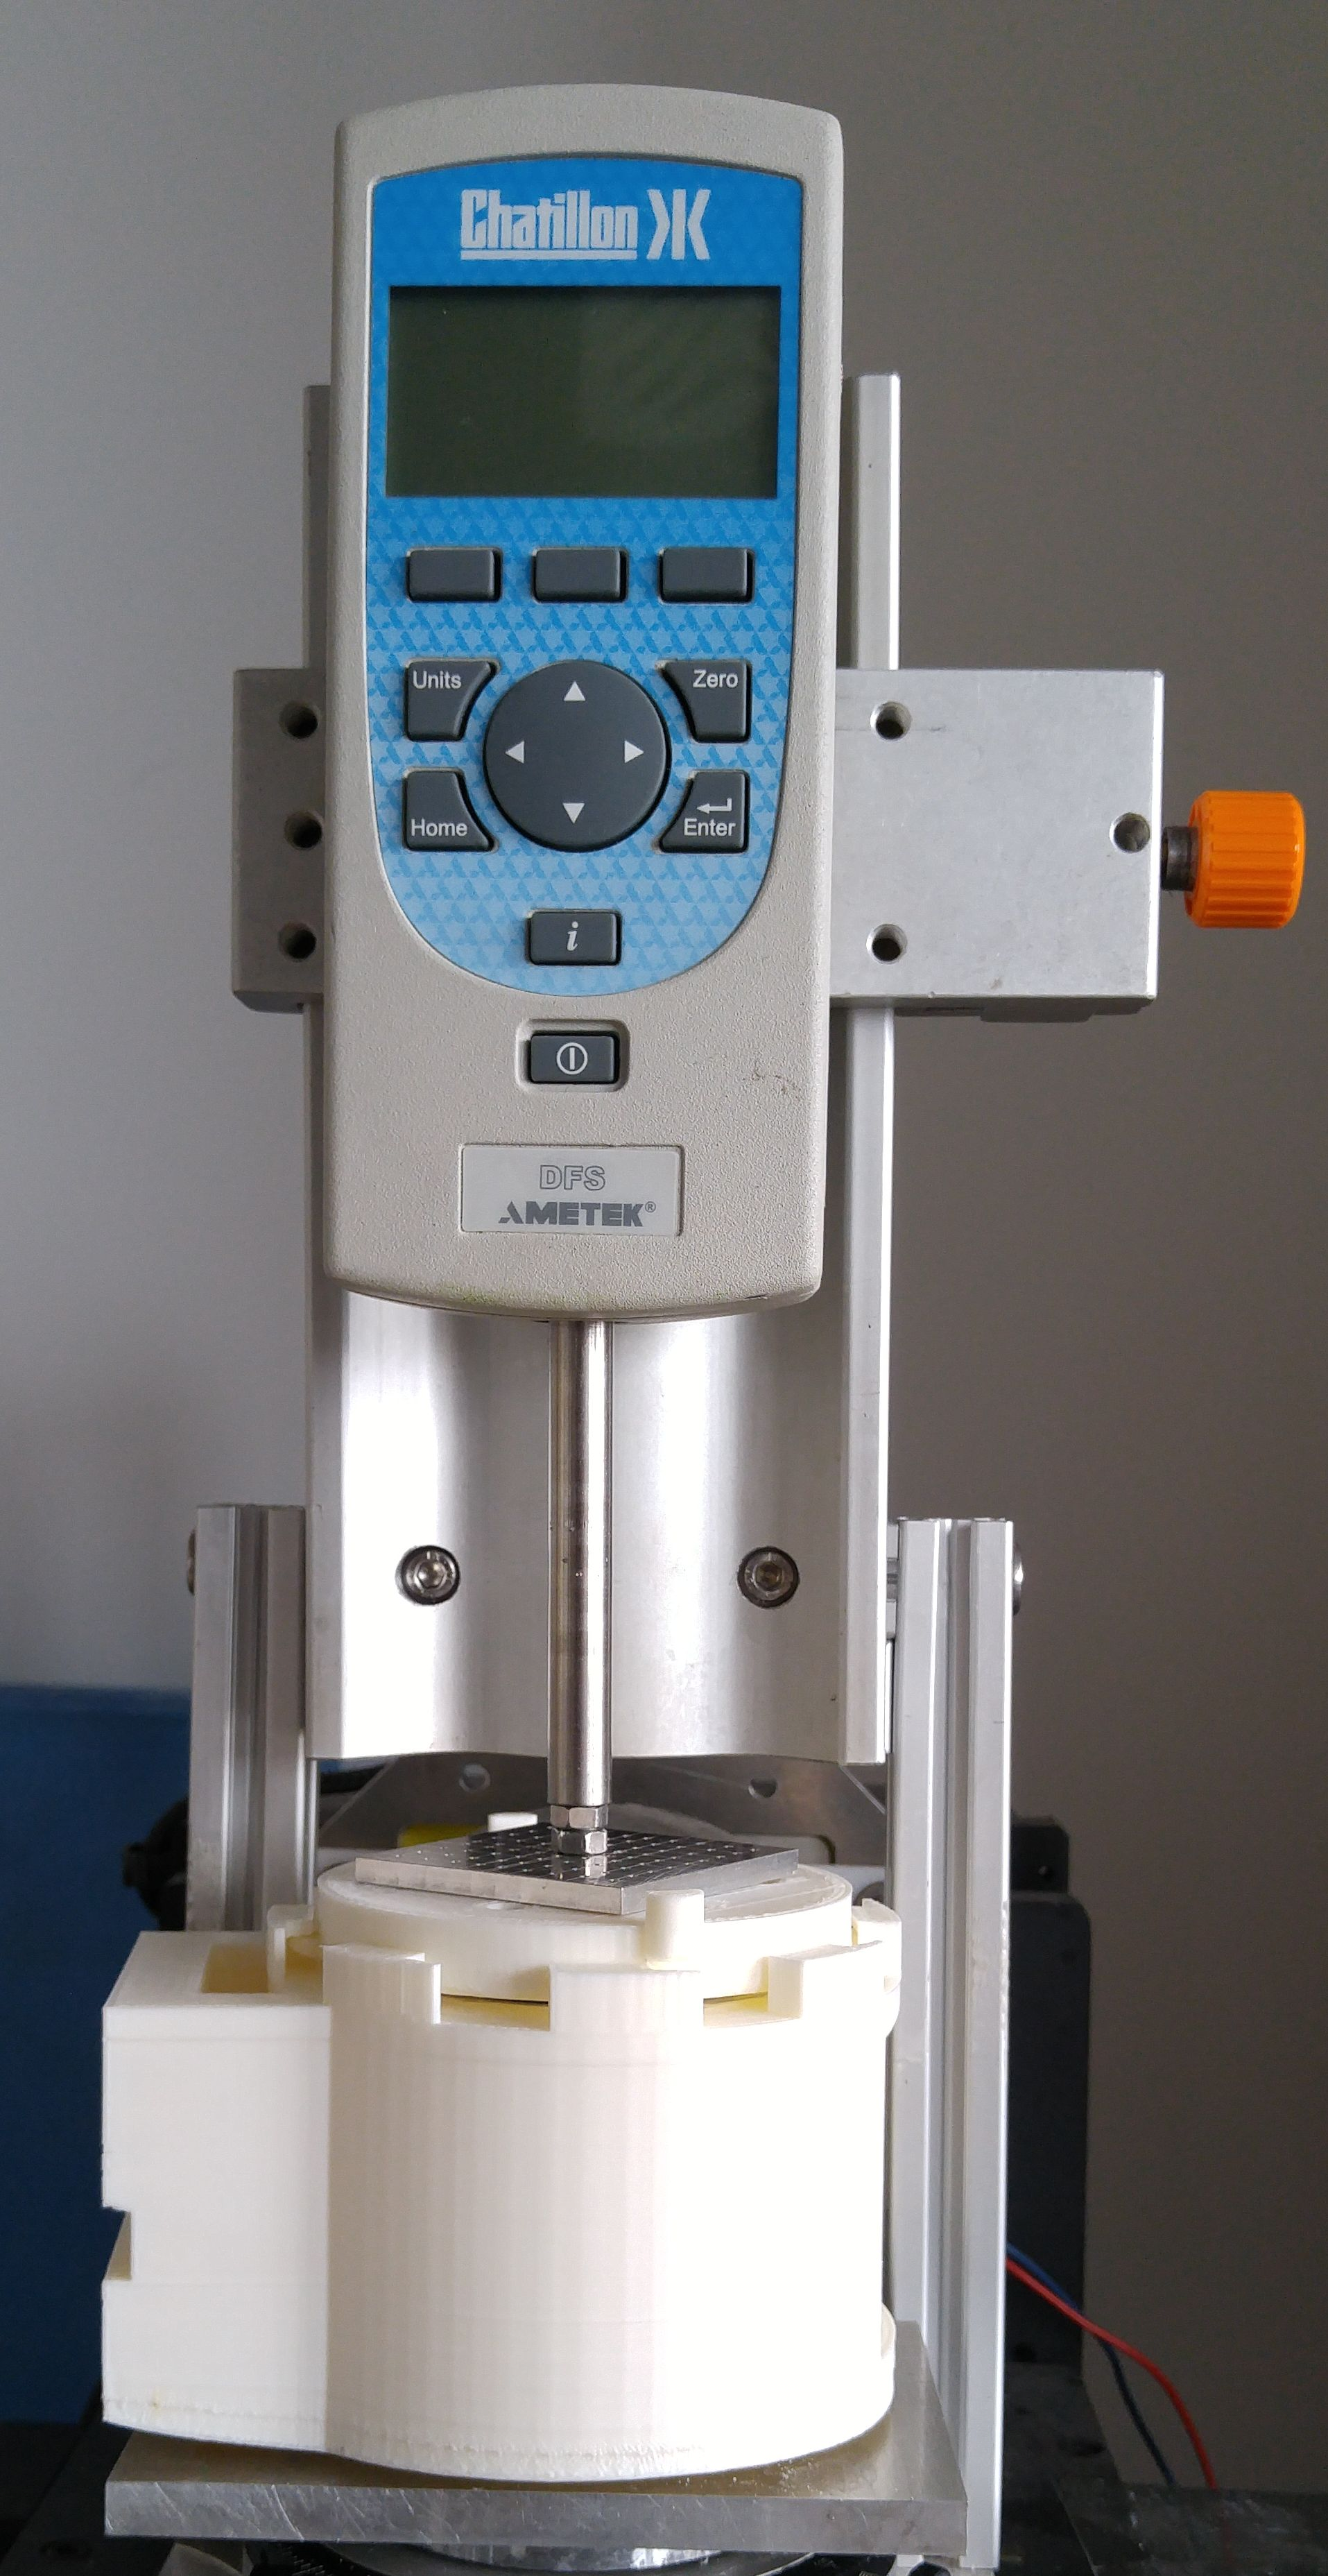
\includegraphics[scale=0.5]{Messmethode_Anpressung.png}
		\caption{Messaufbau um den benötigen Druck zur Arretierung des Röhrchenhalteres zu messen}
	\end{center}
\end{figure}

Um die Festigkeit der einzelnen Arretierungspunkte zu messen, wurde ein T-Stück in das Kraftmessgerät geschraubt und dann das T-Stück in den Arretiungspunkt eingehakt. Anschließend wurde am Anschlusszylinder gezogen und die Kraft protokolliert, bei dem ein Knacken des Materials zu vernehmen war.

\begin{figure}[h]
	\begin{center}
		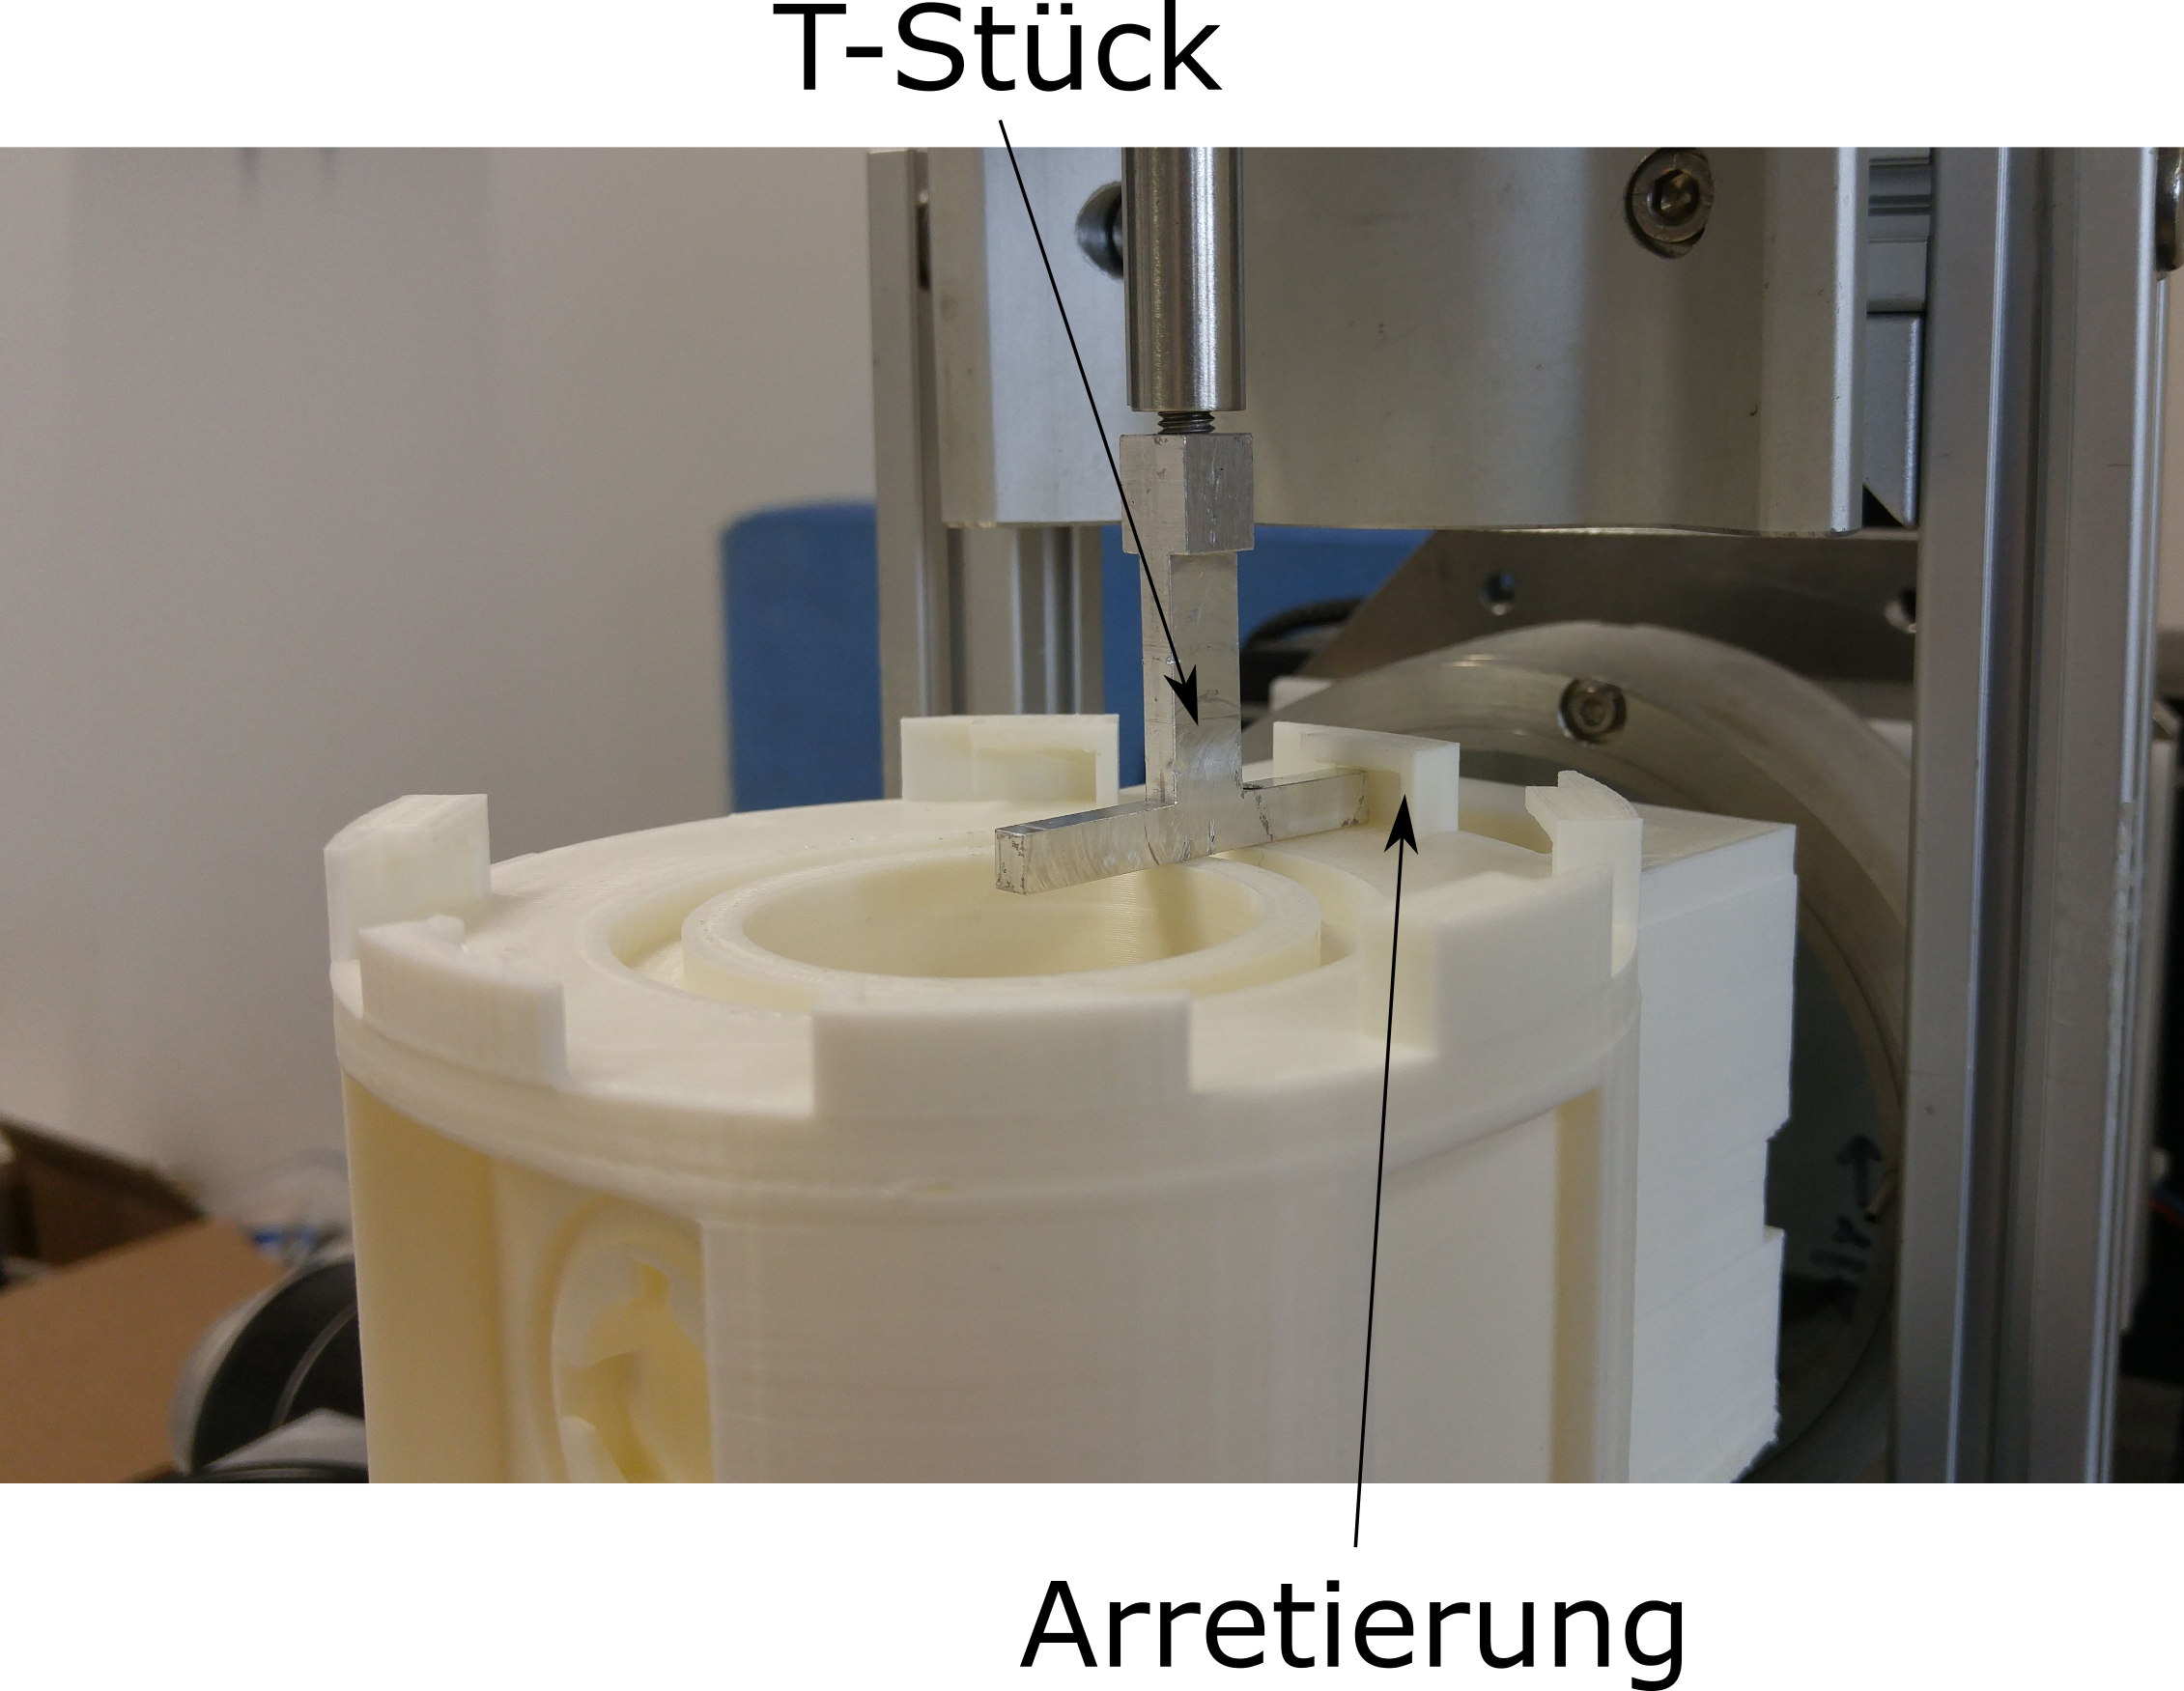
\includegraphics[scale=0.6]{Messmethode_Zugkraft.png}
		\caption{Das T-Stück wird in die Arretierung gehakt und dann daran gezogen, um zu ermitteln wie hoch die maximal ausübbare Kraft zu bestimmen}
	\end{center}
\end{figure}

Weiterhin wurde berechnet wie viel Kraft nötig wäre, damit sich der Röhrchenhalter von selbst aus der Arretierung löst. Bei einer Kraft von \SI{60}{N} und einem Haftreibungskoeffizienten von 0,3 (Kunststoff auf Kunststoff, \cite{Schumann2011}) ergibt sich:
\begin{align*}
F_R = \SI{60}{N} \cdot 0,3 = \SI{18}{N}
\end{align*}
Eine Kraft dieser Größenordnung tritt bei unseren Versuchsbedingungen nicht auf, daher kann man die Möglichkeit einer Selbstlösung vernachlässigen.

\begin{figure}[h]
	\begin{minipage}[hbt]{6.0cm}
		\centering
		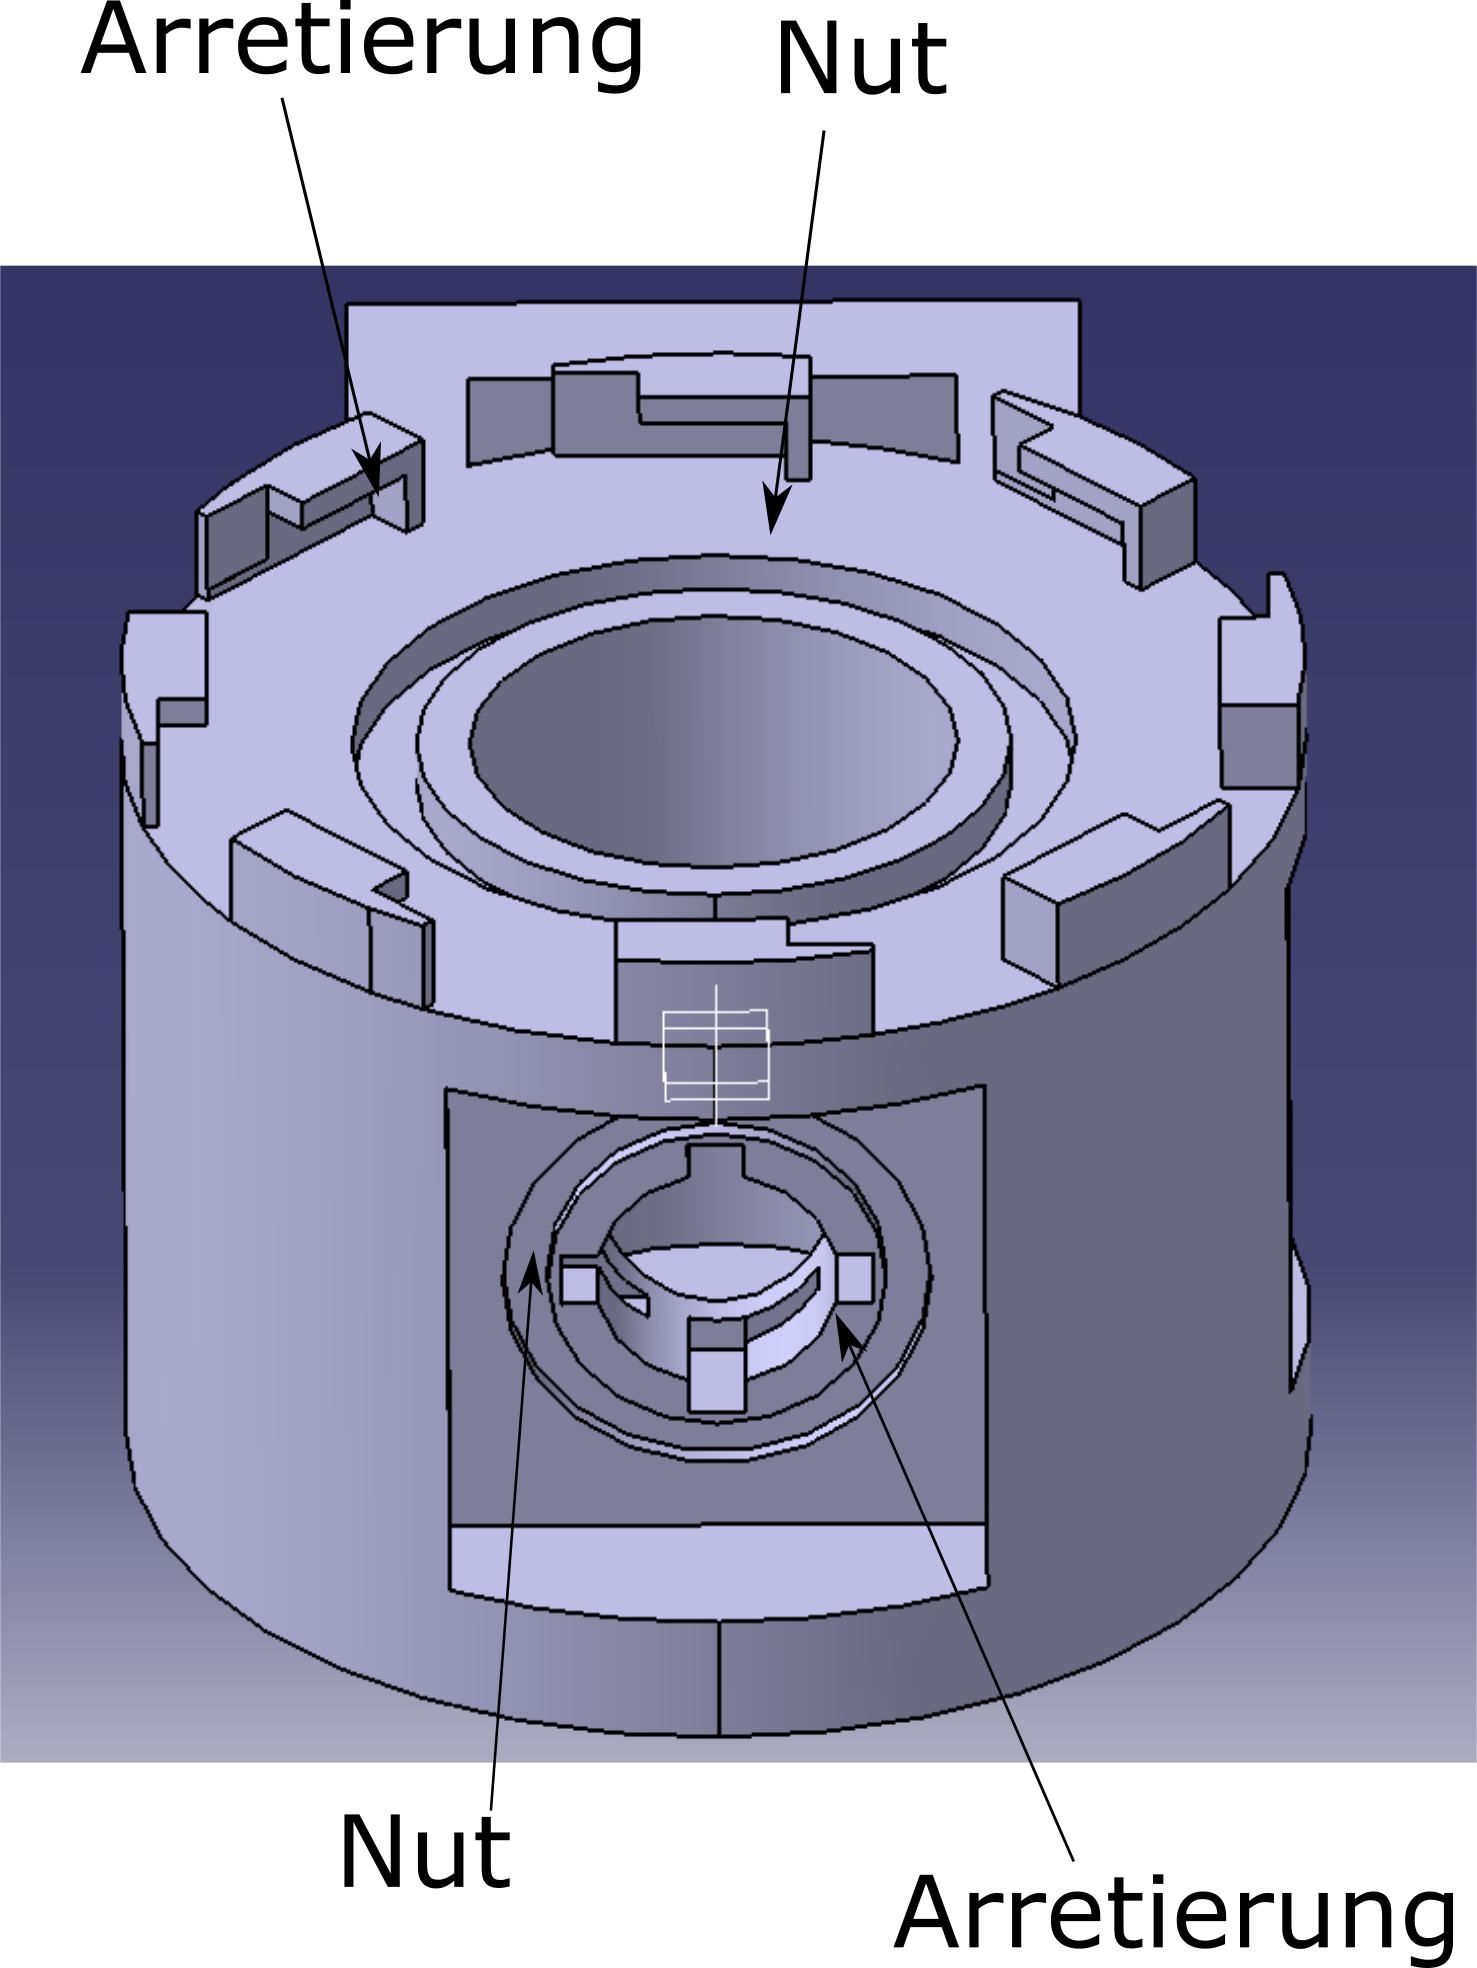
\includegraphics[width=6.0cm]{Zylinder_frontal.png}
	\end{minipage}
	\hfill
	\begin{minipage}[hbt]{7cm}
		\centering
		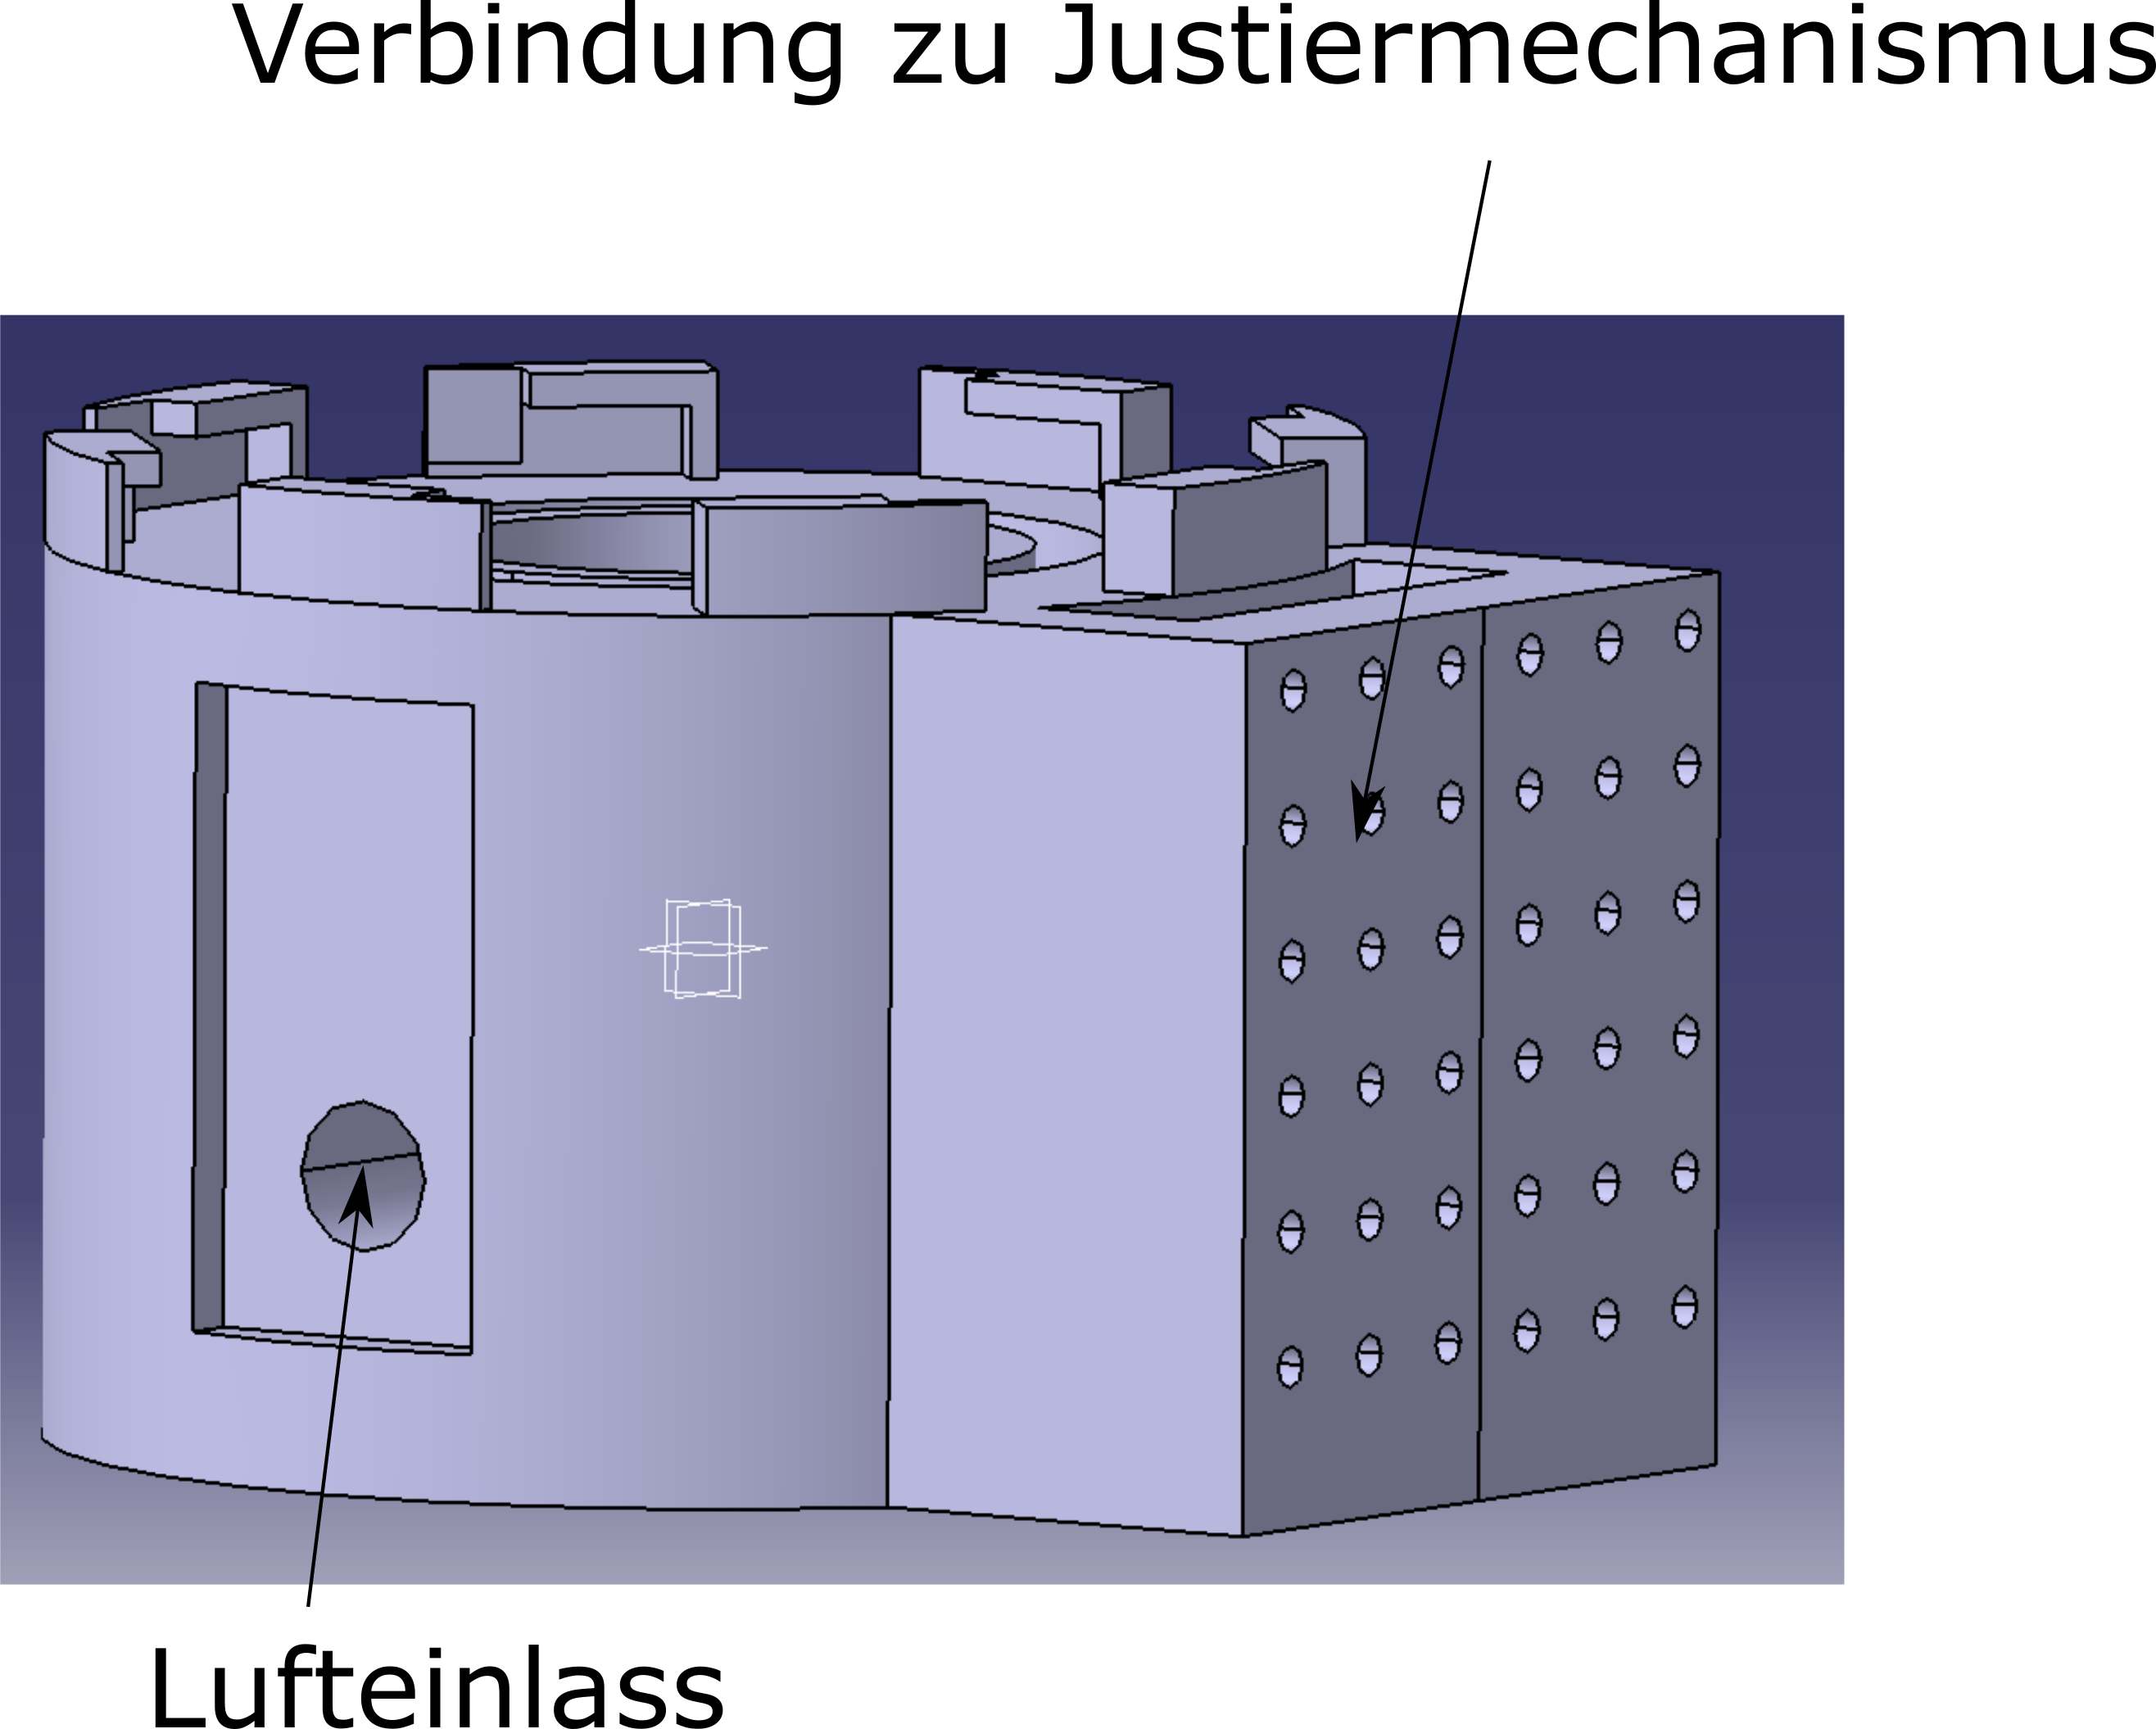
\includegraphics[width=7cm]{Zylinder_seitlich.png}
	\end{minipage}
\end{figure}

In der Frontansicht sieht man den Einlass mit Arretierung für den Ionisator. Zur Montage wird die Spitze des Ionisator in einen Adapter gesteckt und dieser Adapter mittels drehen arretiert. Die Luftdichtheit wird durch einen O-Ring aus Gummi (Shore Härte 50) erreicht. In der Seitenansicht wird der Anschluss für das Gassystem sichtbar. Hier wurde ein Swagelockverbinder mit Gummi O-Ring in das Plastik geschraubt und der Adapter für den Bunaschlauch daran angeschlossen.

\subparagraph{Veränderungen zur Sicherstellung der Luftdichtheit}
\hfill \\

Erste Messversuche mit dem 3D gedruckten Anschlusszylinder zeigten, das \SIrange{40}{50}{\%} des Volumenstroms auf unbekanntem Weg verloren gehen. Daher wurde das gesamte Wirbelbett in Wasser getaucht, um auf diese Weise die Leckstellen zu identifizieren. Dabei stellte sich heraus, dass das 3D gedruckte Plastik an sich undicht ist. Hauptsächlich strömte die Luft an den Löchern für die Befestigung an der Halteplatte und an überhängenden Kanten aus. Die Leckstellen können auf Grund der schwankenden Druckqualität von Druck zu Druck variieren, allerdings wurden Leckstellen vornehmlich an Kanten und Löchern und nicht an großen durchgehenden Flächen beobachtet. \\
Auf Grund dieser Erkenntnisse wurde beschlossen das Design des Anschlusszylinders so abzuändern, das dieser in der Werkstatt aus Aluminium (Was????) fräßbar ist. Dazu wurde der bisherige Arretiermechanismus und die Verbindung zum Justiermechanismus weggelassen, da dies nur sehr aufwändig zu fertigen ist.

\begin{figure}[h]
	\begin{center}
		\includegraphics[scale=0.5]{Schnitt_AnschlusszylinderV2.png}
		\caption{In das M12x1 Gewinde wird der Swagelokadapter geschraubt, dabei dichtet die Dichtung des Adapters mit der Auflagefläche zusätzlich ab. Die M6 Gewinde dienen zur Arretierung des Röhrchenhalters. Die Nut nimmt die gleiche Dichtung auf wie schon weiter oben beschrieben.}
	\end{center}
\end{figure}

Zudem stellte sich während der Messungen heraus, das der verwendete Luftionisator (Haug Static Line LC) nicht den gewünschten Effekt erzielt, daher wurde dieser Anschluss bei der Ausführung in Aluminium ebenfalls weggelassen. Um den Anschlusszylinder trotzdem mit dem Justiermechanismus zu verbinden, wird dieser Teil weiterhin im 3D Drucker gedruckt und anschließend mit zwei Komponentenkleber (UHU Plus, 2-K-Epoxidkleber) an den Anschlusszylinder angeklebt.

\subsection{Röhrchenhalter}

\paragraph{Umsetzung}

\hfill \\

Der Röhrchenhalter besteht aus drei Teilen, eins dient zur Verbinung mit dem Anschlusszylinder und das andere sorgt dafür, dass die Dichtung an Ort und Stelle gehalten wird. 

\begin{figure}[h]
	\begin{center}
		\includegraphics[scale=0.5]{Schnitt_Roehrchenhalter.png}
	\end{center}
\end{figure}

Beide Auflagestellen des O-Rings sind zudem mit Silikon beschichtet, um einen möglichst dichten Abschluss zu gewährleisten.
Diese Teile werden durch sechs M6 Schrauben verbunden, damit die Kraft auf den dichtenden O-Ring möglichst gleichmäßig verteilt ist. \\

\begin{figure}[h!]
		\begin{center}
			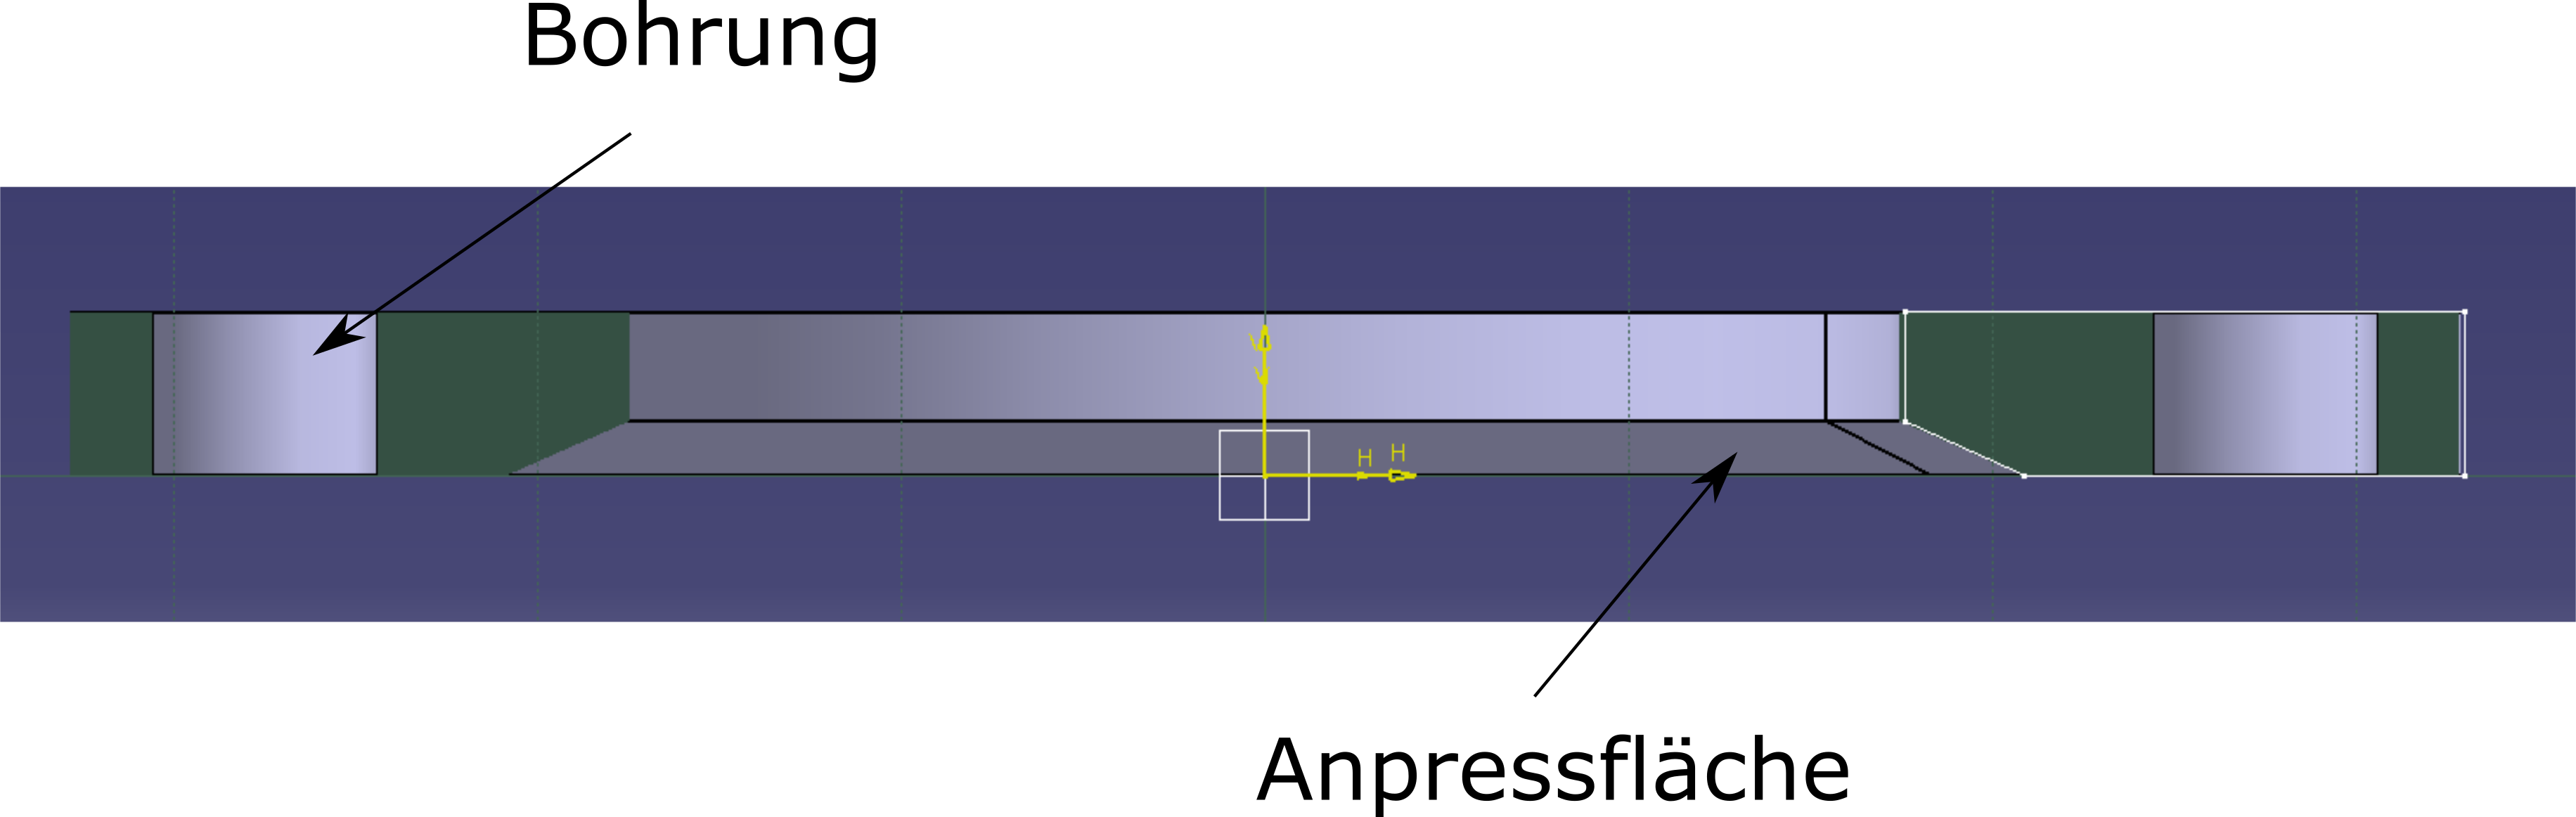
\includegraphics[scale=0.5]{Schnitt_Deckplatte.png}
			\caption{Die Anpressfläche ist mit Silikon beschichtet und sorgt für einen dichten Kontakt zum O-Ring}
		\end{center}
\end{figure}

\newpage

Die Kraft, die eine einzelne Schraube auf den Ring ausübt, kann aus dem angelegten Drehmoment berechnet werden:

\begin{align*}
	M_A &= M_K + M_G = F_{VM} \cdot \mu \cdot r_A + F_{VM} \cdot \frac{d_2}{2} \cdot \tan\left( \alpha + \phi' \right) \\
	&= \left( F_{Kl} + F_A \cdot \left( 1 - \Phi \right) + F_Z \right) \cdot \mu \cdot r_A + \left( F_{Kl} + F_A \cdot \left( 1 - \Phi \right) + F_Z \right) \cdot \frac{d_2}{2} \cdot \tan\left( \alpha + \phi' \right) \\
	\intertext{Man geht davon aus, das kein Setzverhalten eintritt bzw. dieses vernachlässigbar ist. Zudem kann man nur die resultierende Kraft bestimmen:}
	&= F_{res} \cdot \left( \mu \cdot r_A  + \frac{d_2}{2} \cdot \tan\left( \alpha + \phi' \right) \right) \\
	\intertext{Es wird das Moment gemessen und daraus die Kraft berechnet:}
	F_{res} &= \frac{M_A}{ \mu \cdot \frac{d_3 + D_B}{4}  + \frac{d_2}{2} \cdot \tan\left( \alpha + \phi' \right)}
	\intertext{Man kann $d_2$, $d_3$ und $\alpha$ aus der Tabelle XX im Anhang ablesen. Der Reibwert $\mu$ wird mit $\mu = \SI{0,325}{}$ Quelle!! angenommen. $\phi'$ berechnet man entsprechend der Formel:}
	\phi' &= \arctan\left( \frac{\mu}{\cos\left( \frac{\beta}{2} \right)} \right) 
	\intertext{Dabei ist $\beta$ der Standartflankenwinkel von $\SI{60}{^\circ}$ eines ISO-Gewindes.}
	&= \arctan\left( \frac{0,325}{\cos(\SI{30}{^\circ})} \right) = \SI{20,57}{^\circ}
	\intertext{Bei einem gemessenen Drehmoment (mittels CDI Werameter 7131A) von $M_A = \SI{1}{Nm}$, ist die wirkende Kraft einer Schraube:}
	F_{res} &= \frac{\SI{1}{Nm}}{0,325 \cdot \frac{\SI{4,773}{mm} + \SI{6}{mm}}{4} + \frac{\SI{5,35}{mm}}{2} \cdot \tan(\SI{3,405}{^\circ} + \SI{20,57}{^\circ})} = \SI{0,482}{N}
\end{align*}

Bei sechs Schrauben erhält man eine Gesamtkraft von $F_{ges} = \SI{2,904}{N}$ Dies reicht auch bei einem Probenrohrdurchmesser von \SI{40}{mm} aus, um eine luftdichte Verbindung zu erreichen. Zudem ist man mit dieser Kraft deutlich unter der Belastungsgrenze von ABS, die bei ca \SI{44}{N/mm} (ISO 527, \cite{C.Dallner2006} \cite{ThyssenPlastics}) liegt.

Der dritte Teil des Halters ist der Stabilisator und sorgt dafür, dass das Röhrchen nicht seitlich verkippt werden kann und es dadurch zu Undichtigkeiten kommt. Damit diese Halterung nicht für jedes Röhrchen separat montiert werden muss, wurde ein universelles Ringsystem entworfen. Das Basisteil wird am Schanier festgeschraubt und hat $\SI{40}{mm}$ Durchmesser. In das Basisteil können nun weitere Ringe eingesetzt und durch verdrehen arretiert werden, damit auch die Durchmesser $30,20,5\SI{}{\ mm}$ einen guten Halt haben.

	\begin{figure}[h]
		\begin{minipage}[hbt]{7.4cm}
			\centering
			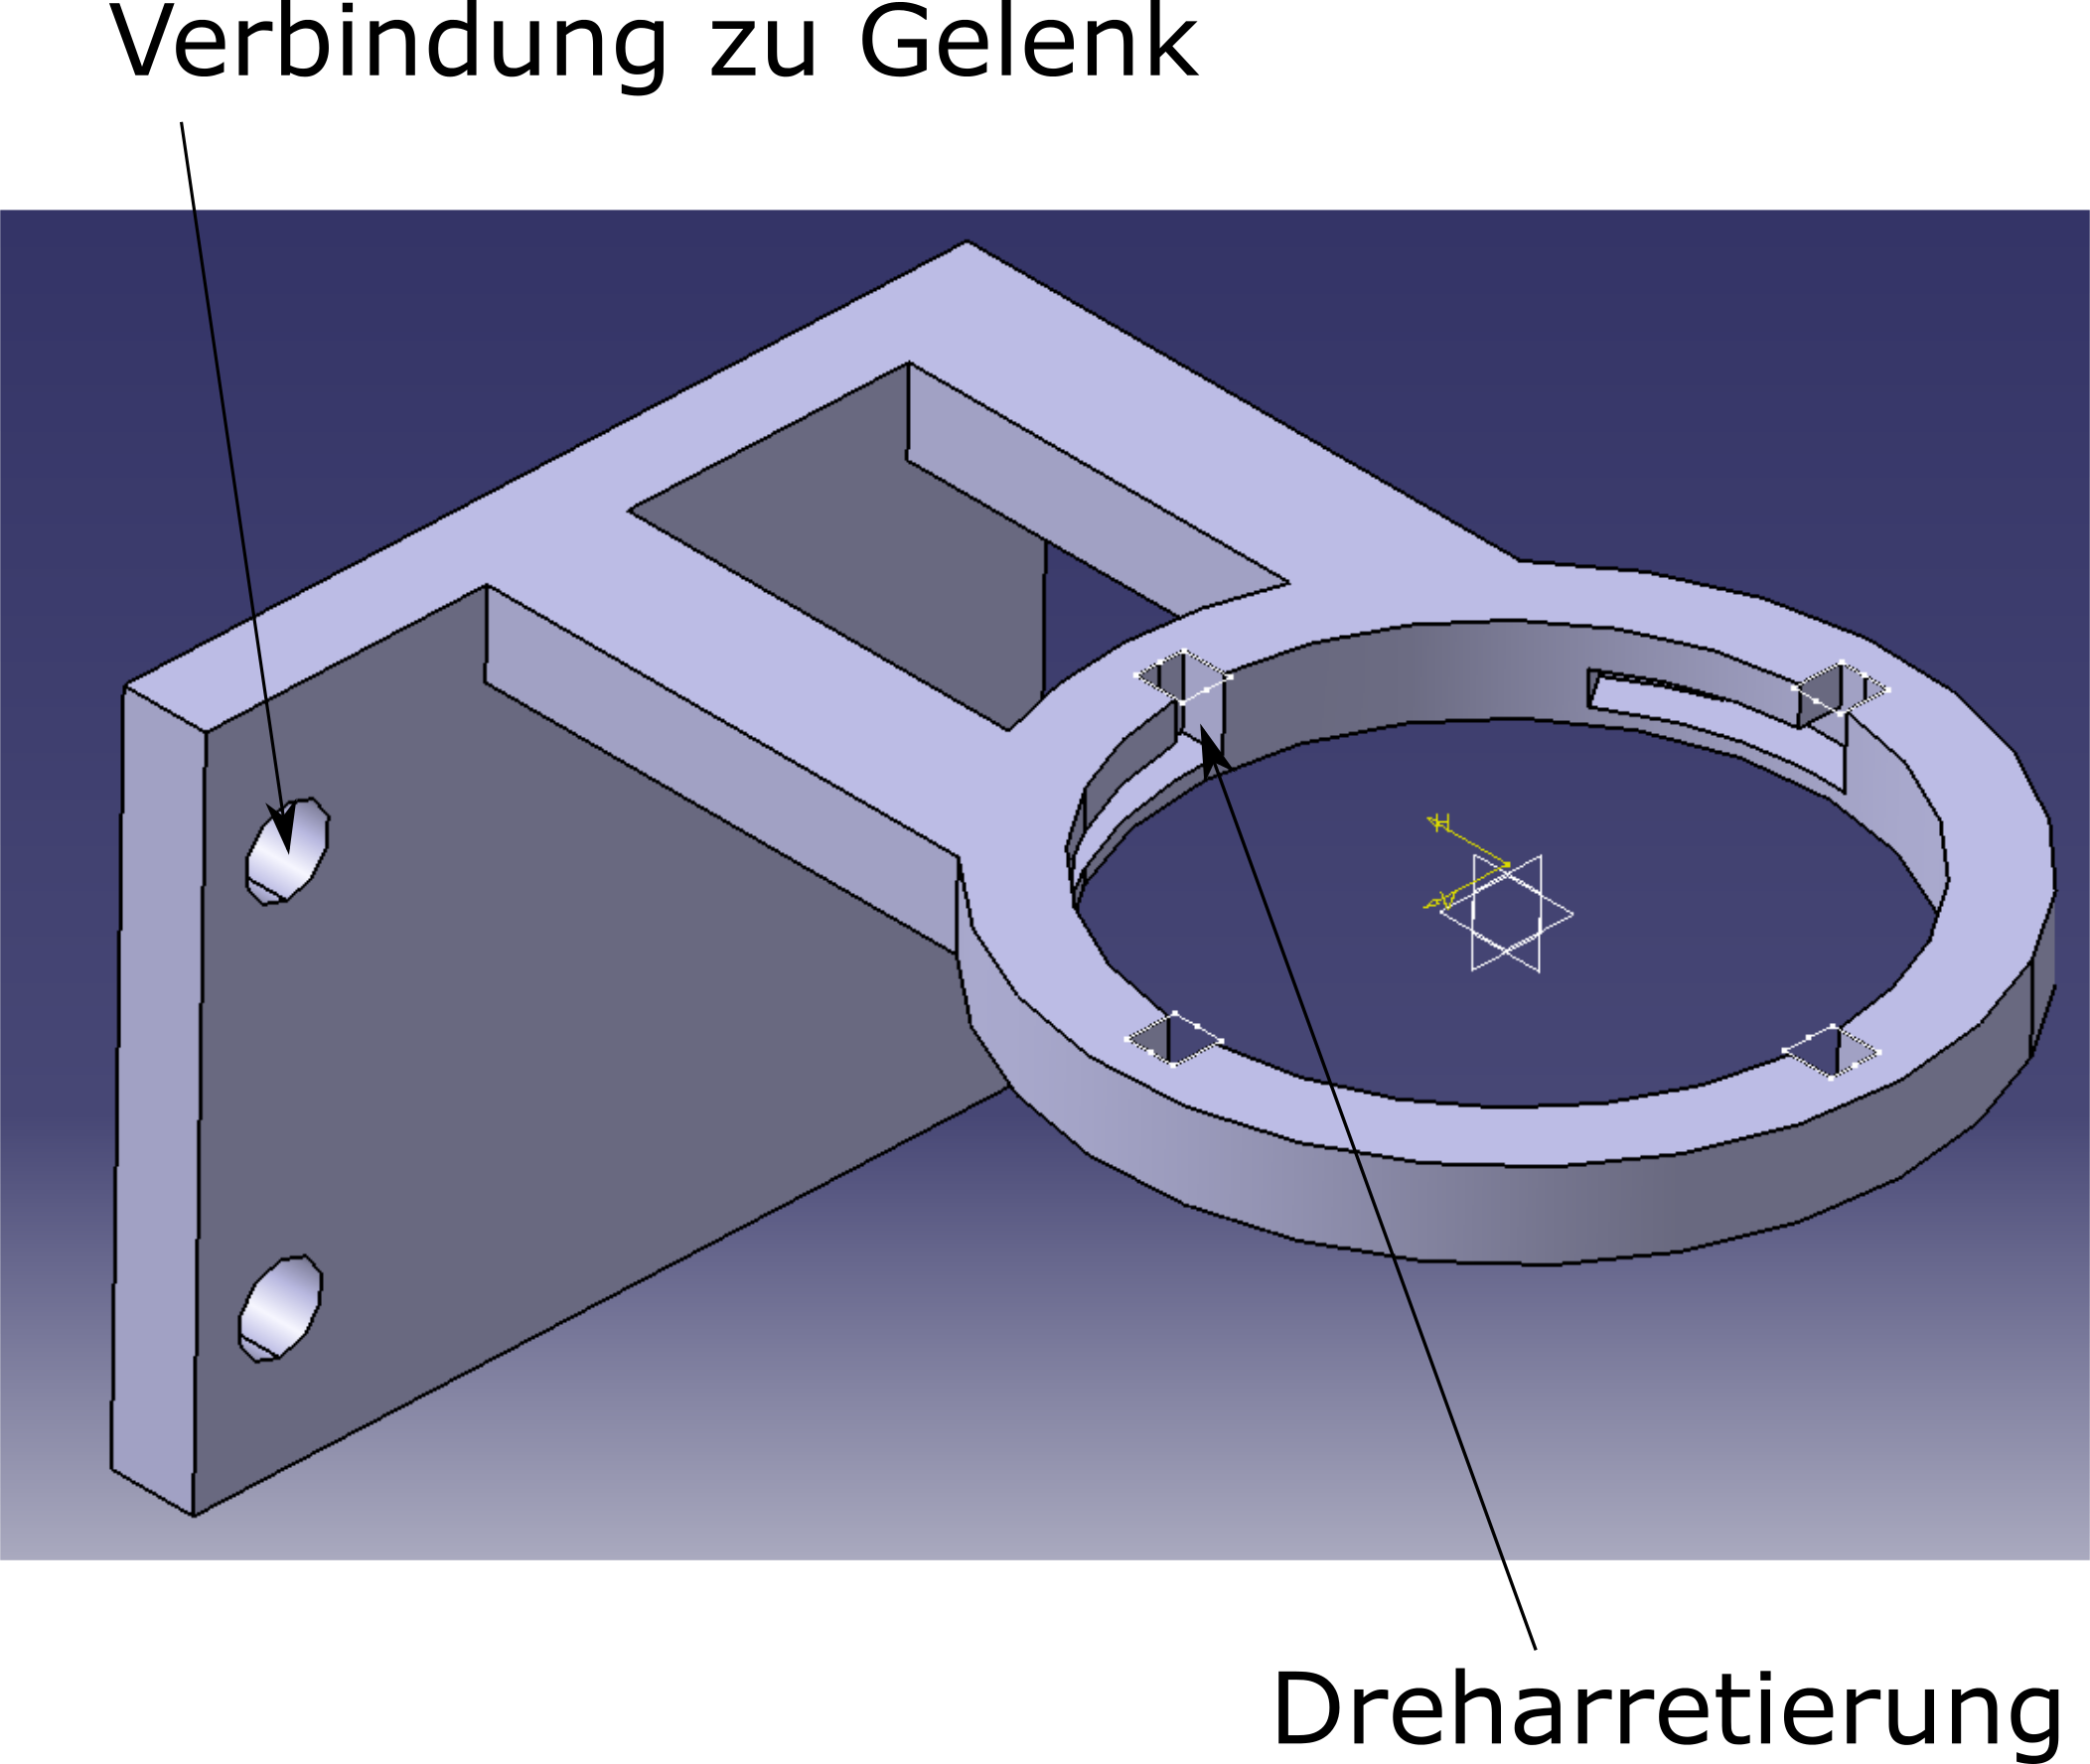
\includegraphics[width=7.4cm]{Basishalter.png}
			\caption{Schwenkbarer Halter der mit Einsätzen für alle möglichen Röhrchendurchmesser angepasst werden kann}
		\end{minipage}
		\hfill
		\begin{minipage}[hbt]{5.7cm}
			\centering
			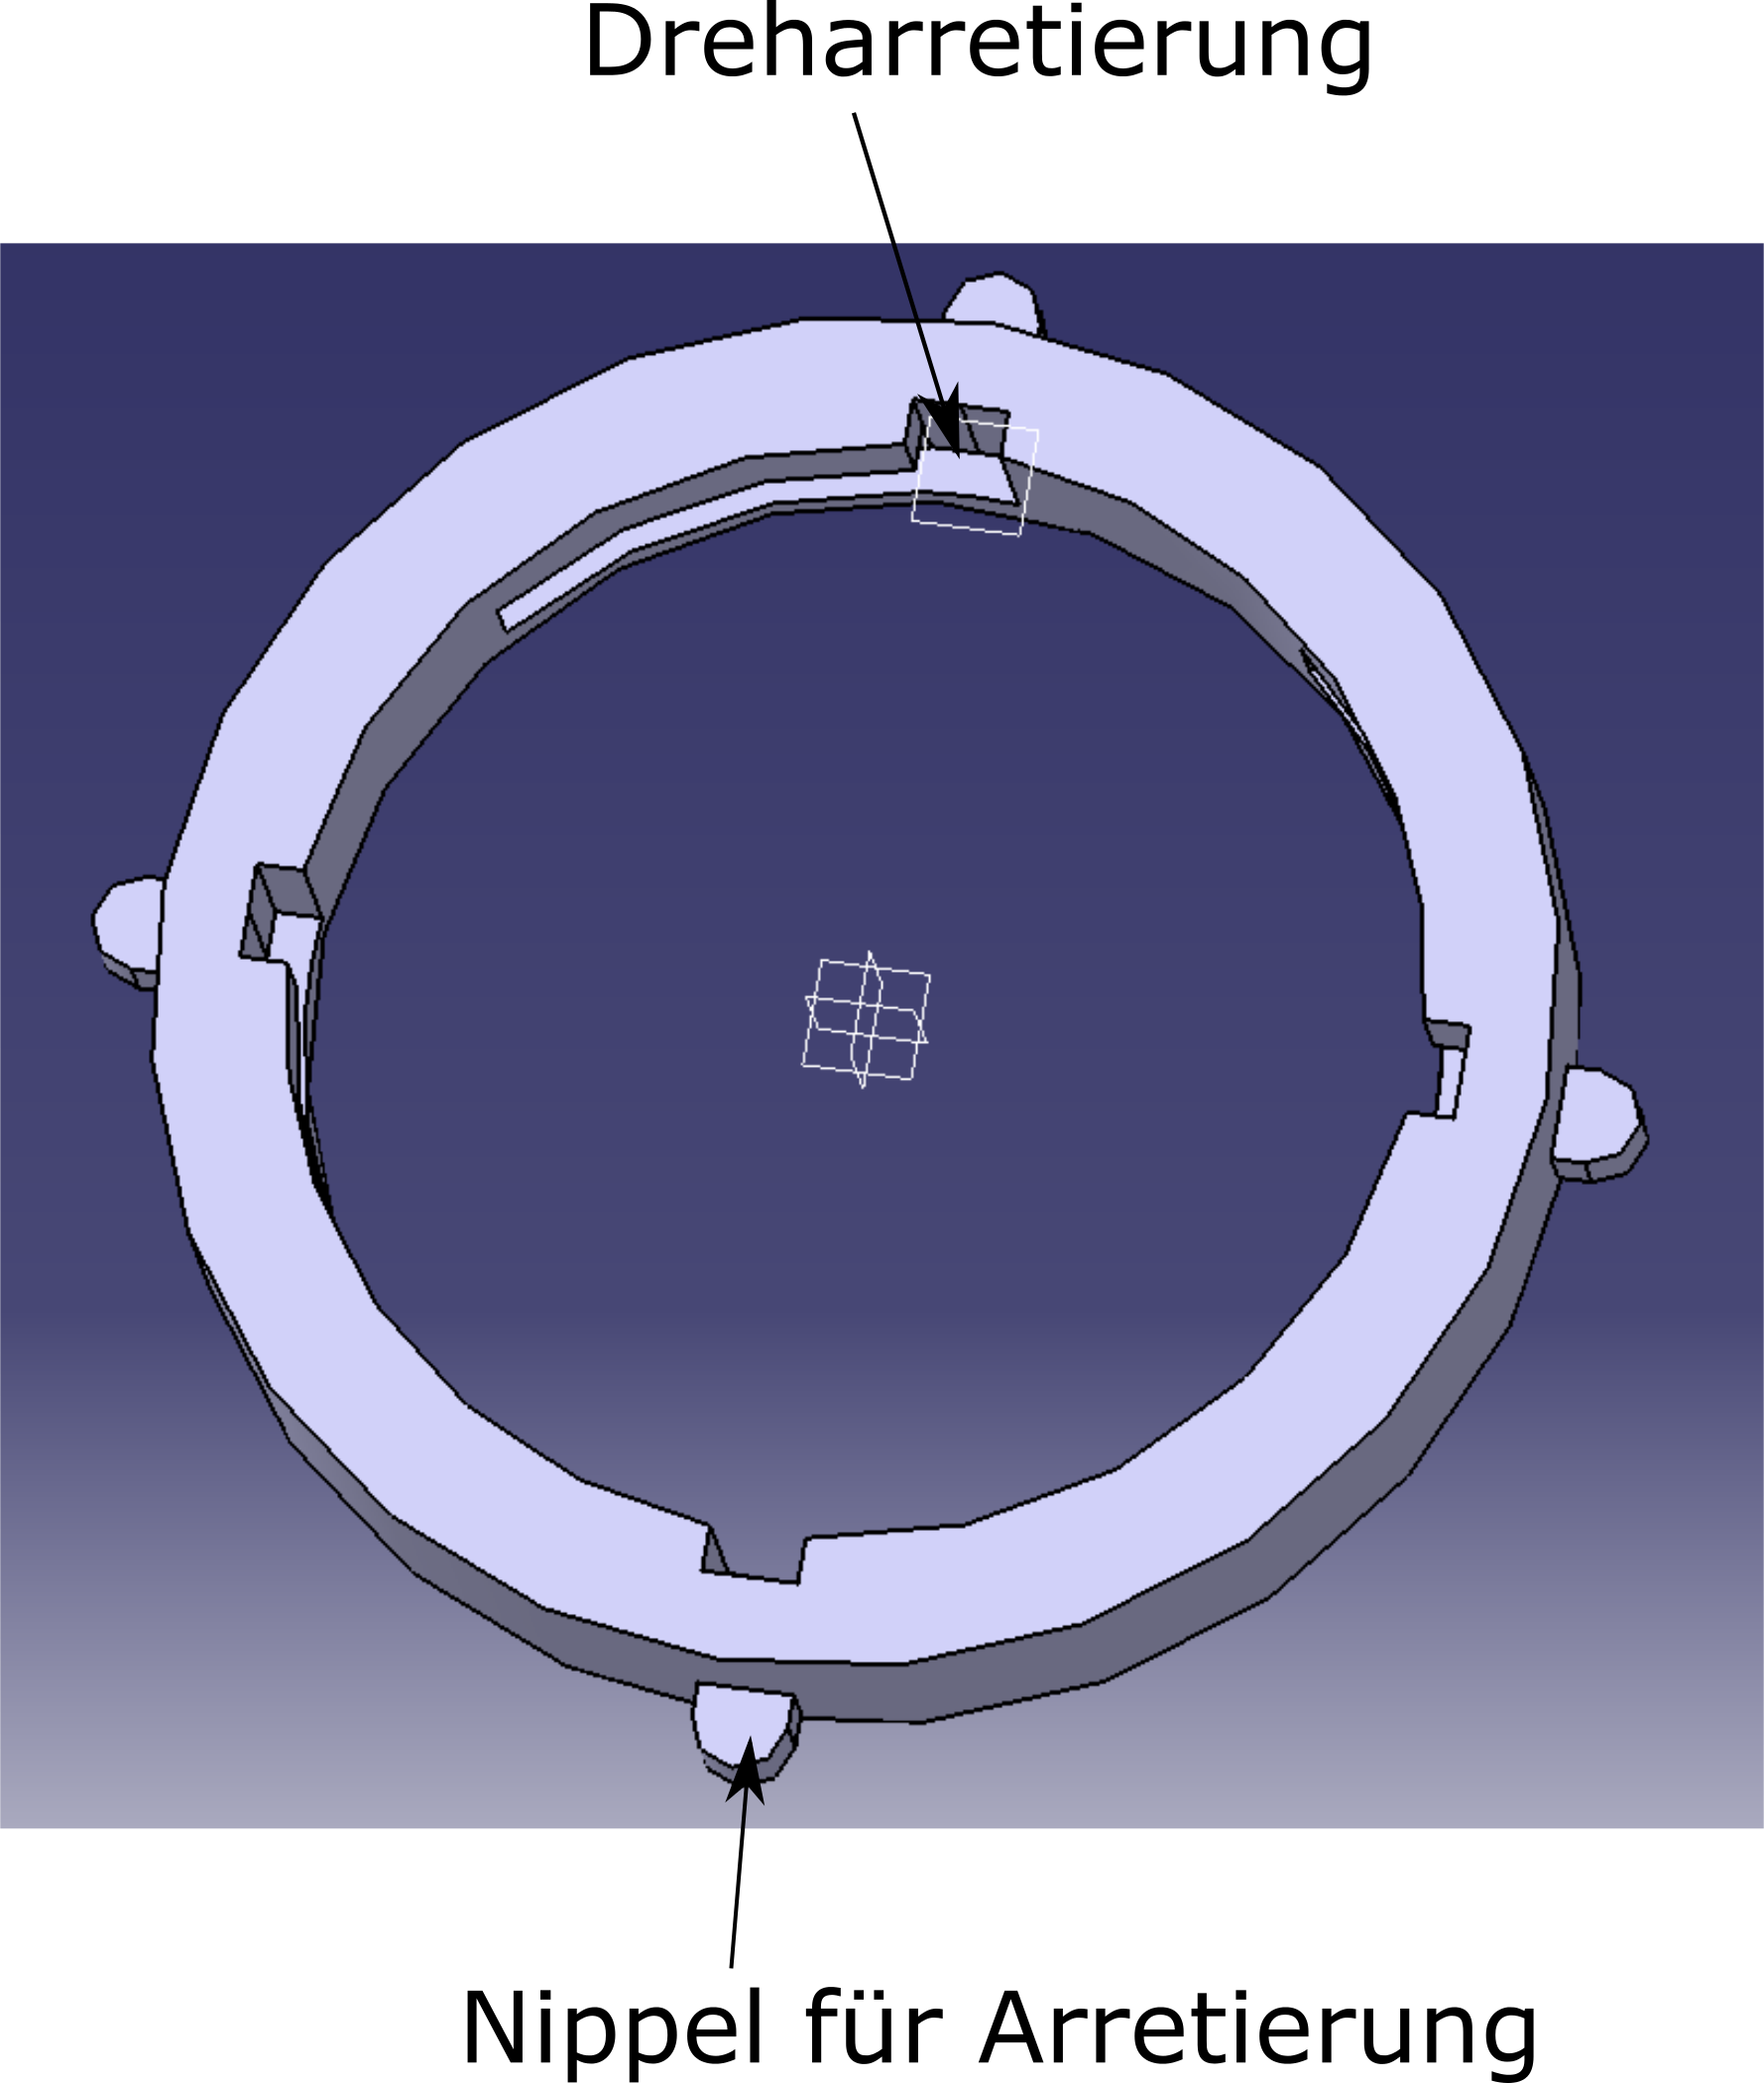
\includegraphics[width=5.7cm]{Basishalter_Einsatz.png}
			\caption{Einsatz für Röhrchen mit \SI{30}{mm} Innendurchmesser}
		\end{minipage}
	\end{figure}
	
\subparagraph{Anpassungen an gefräßten Anschlusszylinder}
\hfill \\

Wegen der Veränderungen am Anschlusszylinder musste der Röhrchenhalter daran angepasst werden. Dazu  wurde der ursprüngliche Mechanismus zur Arretierung entfernt und stattdessen sechs Durchgangsbohrungen eingefügt, damit der Halter von oben auf den Anschlusszylinder geschraubt werden kann.

\begin{figure}[h!]
	\begin{center}
		\includegraphics[scale=0.6]{Schnitt_RoehrchenhalterV2.png}
		\caption{}
	\end{center}
\end{figure}


\subsection{Halterung Wirbelbett}

Sowohl für den Aufbau im Labor als auch für den Aufbau im Lichtstreuaufbau, wurde eine Halterung benötigt. Im folgenden werden die beiden Halterungen vorgestellt.

\subsubsection{Lichtstreuaufbau}


\paragraph{Anforderungen}

\hfill \\
Die Aufgabe bestand darin, das Wirbelbett so in den Aufbau zu integrieren, sodass weder die Rotationsfähigkeit vermindert, noch der Aufbau verändert wird. Zudem sollte die Höhe des Wirbelbetts rudimentär geändert werden und die Position in der Horizontalen im Submilimeterbereich eingestellt werden können. 


\paragraph{Umsetzung}
\hfill \\
Um den Anforderungen gerecht zu werden, wurde eine Konstruktion aus zwei L-förmigen Teilen gewählt. 

\begin{figure}[h]
	\begin{minipage}[hbt]{7cm}
		\centering
		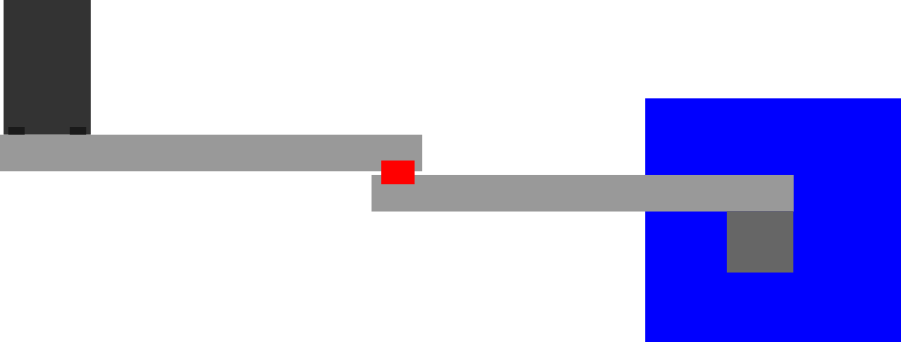
\includegraphics[width=7cm]{Halterung_Lichtstreu_Vogel.png}
		\caption{Draufsicht}
	\end{minipage}
	\hfill
	\begin{minipage}[hbt]{7cm}
		\centering
		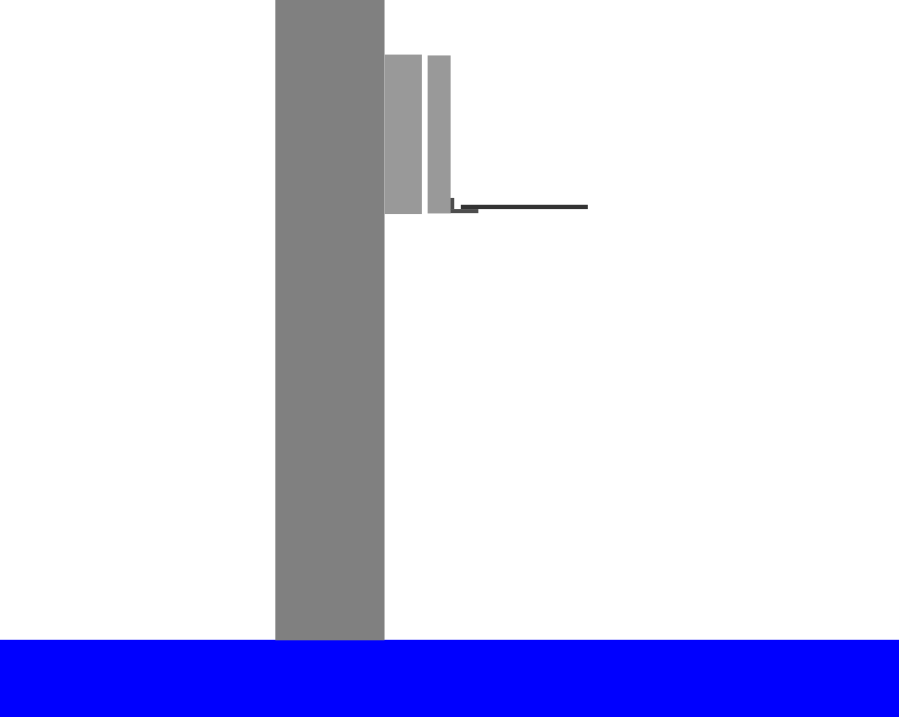
\includegraphics[width=7cm]{Halterung_Lichtstreu_Seite.png}
		\caption{Seitenansicht}
	\end{minipage}
\end{figure}


In der Draufsicht sieht man, das zum Verschieben nach links und rechts zwei durch eine Laborklemme (rot) gegeneinander verschiebbare Träger genutzt wurden. Ans Ende es linken Trägers wurde mittels zwei Winkeln die Halteplatte für das Wirbelbett montiert. Auf der Halteplatte kann das Wirbelbett mit der Mikrometerschraube exakt in den Laserstrahl gefahren werden.


\subsubsection{Laboraufbau}

\paragraph{Anforderungen}
\hfill \\
An die Halterungen im Labor gab es lediglich die Anforderung, das sie stabil ist und eine horizontale Ausrichtung des Wirbelbetts ermöglicht.

\paragraph{Umsetzung}
\hfill \\
Die Anforderungen wurden zum einen durch eine Platte auf der der Justiermechanismus des Wirbelbetts festgeschraubt wird erfüllt. Für einen stabilen Stand werden in Platte vier Beine mit Füßen von jeweils \SI{3}{cm} Durchmesser eingeschraubt. Durch den Schraubmechnismus können auch schiefe Arbeitsflächen korrigiert werden.



\begin{figure}[h]
	\begin{center}
	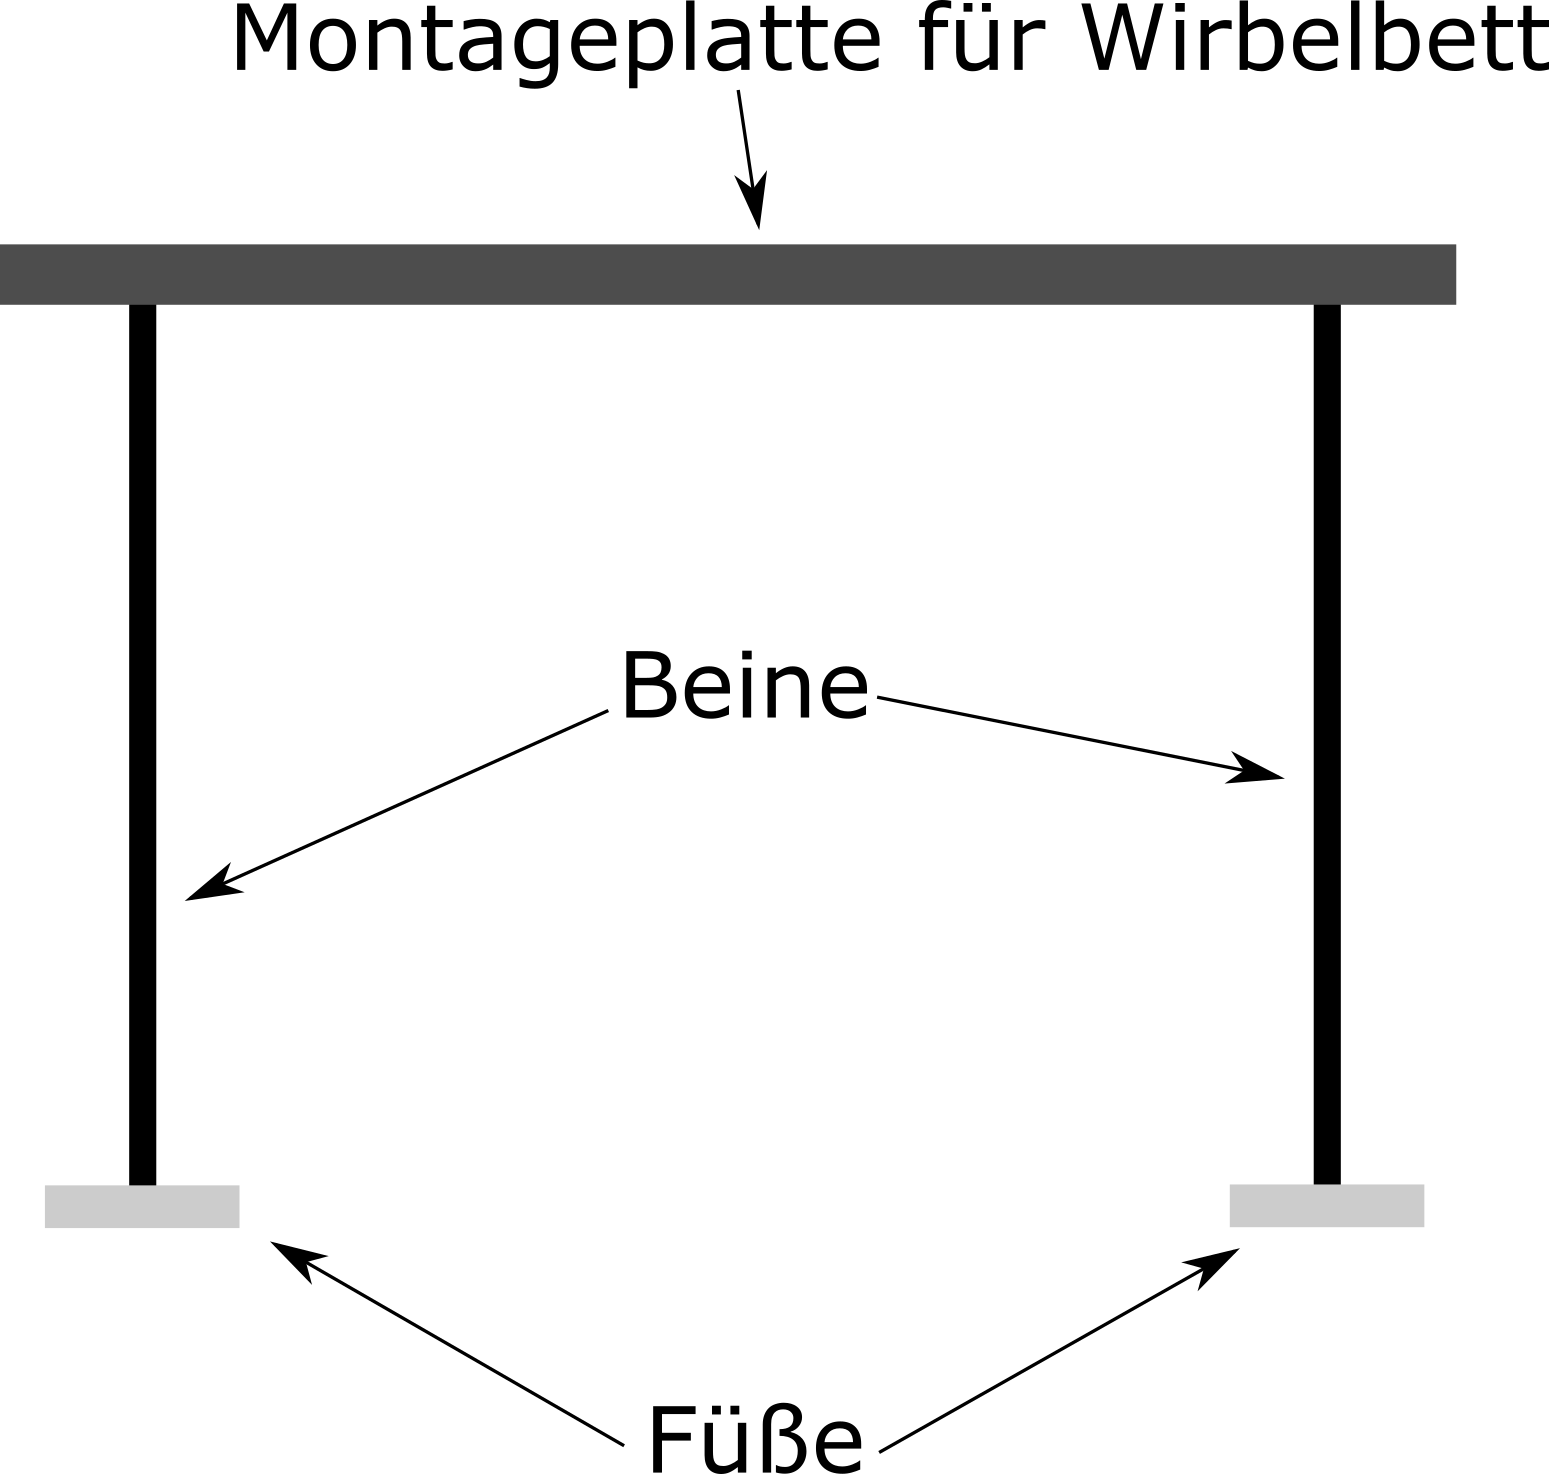
\includegraphics[scale=0.6]{Halterung_Labor_Seite.png}
    \end{center}
\end{figure}




\subsection{Filter}

\paragraph{Anforderungen}
\hfill \\
Das Ziel bestand darin einen Filter zu finden, der, im Gegensatz zu dem vorher verwendeten Schwamm, immer die gleichen Eigenschaften aufweist, auch wenn man ihn austauscht. Zudem muss der Filter durchlässig genug sein um bis zu $\SI{3000}{l/h}$ Luft durchzulassen, ohne zu reißen. Zugleich müssen die Poren fein genug sein, damit die Partikel des kleinsten Granulats nicht hindurch fallen. Außerdem muss der Filter dünn genug sein, damit der die Höhe der Konstruktion nicht negativ beeinflusst, da es beim Lichtstreuaufbeu eine Höhenbegrenzung gibt. Weiterhin musste der Filter hydrophob und antistatisch sein, sodass er bei Zuschaltung des Luftbefeuchters kein Wasser aufnimmt und dadurch verstopft und sich nicht statisch aufläd.


\paragraph{Auswahl}
\hfill \\
Um einen geeigneten Filter zu finden wurde sich mit den Herstellern Merk Millipore, Sartorius und Nitto in Verbindung gesetzt. Am Schluss hatten wie die Auswahl zwischen folgenden Filtern:


\begin{center}
			\begin{tabular}{l|c|c|c}
				& Sartorius & Merck Millipore & Nitto \\
				\hline
				Porengröße [$\mu$m] & 0,45  & 10    & 24 \\
				Dicke[$\mu$m] & 125 & 130 & 500 \\
				Porösität[$\%$] & 75    & 60    & 38 \\
				Luftdurchlass [$l/min \cdot cm^2$] & 20    & 14    & 0,09 \\
				antistatisch & ja    & ja    & ja \\
				hydrophob & ja    & ja    & ja \\
				Material & PVDF\footnotemark[1]  & PTFE\footnotemark[2]  & PE\footnotemark[3] \\
			\end{tabular}	
\end{center}

\footnotetext[1]{Polyvinylidenfluorid}
\footnotetext[2]{Polytetrafluorethylen}
\footnotetext[3]{Polyethylen}

\vspace{0.5cm}

Es wurde sich für die Membran von Sartorius entschieden, weil sie alle Anforderungen erfüllt und in allen Belangen besser ist als die beiden Alternativen. Damit die Membran nicht verrutscht wurde ein jeweils passendes Stück auf die Probenröhrchen geklebt. So ist auch sicher gestellt, das kein Granulat unabsichtlich in den Anschlusszylinder fällt.
Eine weitere wichtige Funktion des Filters ist es einen gleichmäßigen Gasstrom zu erzeugen. Dies wird durch die feine Porung erreicht und kann durch berechnen der Reynoldszahl für die verschiedenen Durchmesser bestätigt werden. Zur Berechnung geht man wieder vom maximalen Gasstrom von $\SI{3}{m^3/h}$ 

\begin{center}
\begin{tabular}{S|S|S}
 {Röhrchendruchesser [mm]}		& {Gasgeschwindigkeit $v_{Gas}$ [m/s]}	& {Reynoldszahl}  \\
	\hline
	40	&	0,88		&  0,025 \\
	\hline
	30	&		1,57	&  0,046 \\
	\hline
	20	&	3,53		&  0,11 \\
	\hline
	5	&	14,15		&  0,41 \\
	\hline
\end{tabular}	
\end{center}

Die Reynoldszahlen sind alle weit unter 2300, also ist die Strömung durch die einzelnen Poren laminar und sorgt damit für eine gleichmäßige Anströmung des Granulats über den gesamten Querschnitt des Röhrchens.

\newpage

\section{Messungen}

In diesem Abschnitt wird die Luftdichtigkeit des Wirbelbetts nachgewiesen, als auch Ergebnisse von Messungen an Granulaten dargelegt.

\subsection{Nachweis der Dichtigkeit}

\paragraph{Messmethode}
\hfill \\
Um die Dichtigkeit möglichst nahe an den realen Messbedingungen zu testen, wurde entschieden, dass man die Volumenströme vor und hinter dem Wirbelbett miteinander vergleicht. Dies hat den Vorteil, dass der Filter auf dem das Granulat liegt einen beständigen Luftwiderstand darstellt und es dadurch, wie auch bei Messungen, zu einem Druckaufbau vor dem Filter kommt. Gegenüber diesem Druck muss die Apparatur mindestens luftdicht sein. Der Messaufbau besteht aus dem üblichen Aufbau, allerdings wurde am oberen Ende des Röhrchens, um den Volumenstrom in ein Messgerät zu leiten, ein modifizierter Röhrchenhalter aufgesetzt. Gemessen wurde mit einem Röhrchen von \SI{20}{mm} Innendurchmesser.

Bild!!!


Der Messablauf bestand darin, das mit dem Massenstromregler Volumenströme vorgegeben wurden, diese wurden direkt vor dem Wirbelbett mit einem Volumenstrommessgerät gemessen und anschließen mit dem selben Gerät hinter dem Wirbelbett erneut gemessen. Da das Volumenstrommessgerät auf dem Bereich von \SIrange{0}{100}{l/h} beschränkt war, wurde nur in diesem Bereich gemessen.


\paragraph{Ergebnisse}
\hfill \\


\subsection{Vermessung verschiedener Granulate}


\newpage

\section{Bewertung}

In diesem Abschnitt soll der Erfolg der einzelnen Arbeitspakete kritisch hinterfragt werden, um Raum zur Optimierung aufzuzeigen. 

\subsection{Elektronik}

Rückblickend wurde die Komplexität der Elektronik unterschätzt, was dazu führte, das sehr lange unklar war welche Teile verwendet werden. Dadurch war es nicht möglich in dem geplanten Zeitfenster ein finales Gehäuse für die Elektronik zu designen. Da der Zeitaufwand für das Design dieses Teils allerdings nicht sehr hoch war, war es ohne Probleme möglich es am Ende des Projekts zu machen. In Zukunft wäre es besser solche Probleme entweder früher zu erkennen oder das Design von vorne herein ans Ende zu stellen. 

\subsection{Gassystem}

Der gewählte Filter erfüllt zwar alle gestellten Anforderungen, bringt aber einen Nachteil mit sich. Trotz planem Filter beim Aufkleben auf das Probenröhrchen, verformt sich dieser im Laufe der Nutzung plastisch. Das führt zu einem zusätzlichen heben und senken des graularen Mediums um bis zu \SI{3}{cm} (im Rährchen mit \SI{40}{mm}  Durchmesser). Dieses Verhalten ist unerwünscht, da sich die Granulate deswegen nicht komprimieren und dann auf ihr Verhalten untersuchen lassen.  

\subsection{Wirbelbett}



\subsection{Nutzung des 3D Druckers}

Durch die Anforderung einen Ionisator im Aufbau unterzubringen, war es nicht möglich ein anderes Material außer Plastik zu verwenden. Zudem konnte eine andere Herangehensweise gewählt werden, statt klassischen Technischen Zeichnungen und FEM, wurde die Methode des evolutionären Druckens gewählt. Das sparte die aufwändigen Simulationen und erlaubte das Testen der designten Teile unter Realbedingungen. Der Nachteil dieser Methode ist neben den  Fehldrucken, die bei ca \SI{10}{\%} lagen, der Overhead an Teilen. Dadurch das man das selbe Teil in verschiedenen Evolutionsstufen druckt, ist man nicht sehr materialsparend. \\
Die Qualität der gedruckten Bauteile war durchweg hoch, besonders die Stabilität ist beachtlich, allerdings dauert es zwei, drei Drucke bis man seinen Modell am Rechner soweit angepasst hat, das der Drucker so druckt, wie man es beabsichtigt. Zudem ist der Drucker anfällig im Bezug auf den Druckuntergrund. Während des Projekts ist das Kaptontape auf der Heizplatte kaputtgegangen und ohne dieses Tape auf der Heizplatte, ist es nicht möglich Teile mit Durchmesser größer als \SI{40}{mm} mit flachem Boden zu drucken. Die Drucke bogen sich und waren somit ungeeignet für dichtende Zwecke eingesetzt zu werden. Weiterhin stellte sich im Rahmen der Messungen heraus, das der gedruckte Anschlusszylinder nicht luftdicht ist. Die genauen Ursachen sind nicht untersucht worden, allerdings werden die nicht optimal miteinander verschmolzenen Außenwände dabei eine große Rollen spielen.


\subsection{Zusammenfassung}








\section{Ausblick}

Der Ausblick ist zweigeteilt, im ersten Teil wird auf das konstruierte Wirbelbett eingegangen und im zweiten Teil über dessen Weiterentwicklung diskutiert. \\

Wie bereits in der Bewertung erwähnt, gibt es noch Raum für Verbesserungen bei einzelnen Komponenten. Dies betrifft zum Beispiel den Filter, der entweder ersetzt oder durch konstruktive Maßnahmen am biegen gehindert werden sollte. In diesem Zusammenhang kann man sich auch nochmal mit der Integration eines Luftionisator beschäftigen, da dies ein interessantes Konzept ist, unser Ionisator allerdings entweder zu wenig Leistung hatte oder der Filter zu wenig Ionen durchließ.
Weiterhin wäre es interessant zu untersuchen, ob und wie es möglich ist die 3D gedruckten Teile luftdicht zu machen. Eine Möglichkeit die erwogen wurde, ist das tränken in Epokzitharz, allerdings wurde sie aus Zeit- und Erfahrungsmangel nicht weiter verfolgt.

Die Weiterentwicklung des Wirbelbetts bestünde darin, es auch mit Wasser betreiben zu können.









